\pdfoutput=1
%% MERIDIAN: arXiv version, generated from paper/meridian.tex.
%% Build: pdflatex meridian && bibtex meridian && pdflatex meridian && pdflatex meridian
%% (TinyTeX: export PATH="$HOME/Library/TinyTeX/bin/universal-darwin:$PATH")
\documentclass[sigconf,nonacm]{acmart}

\usepackage{CJKutf8}
\usepackage{tikz}
\usetikzlibrary{arrows.meta,positioning,fit,calc,shapes.geometric}
\usepackage{subcaption}
\usepackage{booktabs}
\usepackage{multirow}
\usepackage{enumitem}
\usepackage{balance}
\setlength{\emergencystretch}{2em}
\raggedbottom

% Chinese in a Latin paper: Arphic Song for running text, Arphic Kai for quoted verse.
\pdfmapfile{=gbsnu.map}
\pdfmapfile{=gkaiu.map}
\newcommand{\zh}[1]{\begingroup\normalfont\begin{CJK*}{UTF8}{gbsn}#1\end{CJK*}\endgroup}
\newcommand{\kai}[1]{\begingroup\normalfont\begin{CJK*}{UTF8}{gkai}#1\end{CJK*}\endgroup}

% The town's palette, used in the diagrams.
\definecolor{navy}{HTML}{0B2036}
\definecolor{gold}{HTML}{D3A557}
\definecolor{cream}{HTML}{F6EFE2}
\definecolor{rose}{HTML}{C74B5F}
\definecolor{meadow}{HTML}{5F9E5A}
\definecolor{sky}{HTML}{3F7FB3}
\definecolor{merred}{HTML}{D7102F}
\definecolor{jpurple}{HTML}{7B4FD8}
\definecolor{ygreen}{HTML}{3E9A4E}

% A heart drawn in TikZ, so it prints in any PDF viewer (no emoji font needed).
\newsavebox{\heartbox}
\sbox{\heartbox}{\tikz[baseline=-0.32em,x=1.5em,y=1.5em]{\fill[merred]
  (0,-0.42) .. controls (-0.58,0.02) and (-0.56,0.5) .. (-0.27,0.5)
  .. controls (-0.11,0.5) and (0,0.39) .. (0,0.27)
  .. controls (0,0.39) and (0.11,0.5) .. (0.27,0.5)
  .. controls (0.56,0.5) and (0.58,0.02) .. (0,-0.42);}}
\DeclareRobustCommand{\redheart}{\usebox{\heartbox}}
\DeclareRobustCommand{\ini}[1]{\textcolor{merred}{\textbf{#1}}}

\newcommand{\yt}{Yi Town}
\newcommand{\code}[1]{\textnormal{\texttt{\small #1}}}
\newcommand{\dc}[1]{\textsc{D#1}}

\settopmatter{printacmref=false, printccs=false, printfolios=true}
\renewcommand\footnotetextcopyrightpermission[1]{}
\setcopyright{none}

\begin{document}

\title[MERIDIAN]{\texorpdfstring{\textcolor{merred}{MERIDIAN}\hspace{0.18em}\redheart}{MERIDIAN}}
\subtitle{\ini{M}emory-\ini{E}ncoded \ini{R}ituals for \ini{I}ntimacy across \ini{D}istance
in an \ini{I}nteractive, \ini{A}synchronous \ini{N}eighbourhood}

\author{Jingyi Chen}
\authornote{Both authors approved this manuscript and the disclosure of the personal material it describes.}
\affiliation{\institution{Independent Researcher}\city{Shenzhen}\country{China}}
\email{jingyi@jingyifan.love}

\author{Yifan Yang}
\authornote{Corresponding author.}
\affiliation{\institution{Independent Researcher}\city{College Station, Texas}\country{USA}}
\email{yifan@jingyifan.love}

\renewcommand{\shortauthors}{J. Chen and Y. Yang}


\begin{abstract}
How can shared memories become playable structures for partners who live in different time zones,
and what becomes of such a gift once it is in use? We present MERIDIAN, a design case of Yi Town,
a bilingual browser game developed by one member of a long-distance couple as a gift for the
other. Nine levels translate personally meaningful events, places and cultural references into
tasks within a navigable pixel town, framed by a birthday prologue and a fictional wedding. This
second version extends the record by four weeks. Drawing on research through design, we
reconstruct seven design changes from 147 commits, 36 changelog versions and four design
specifications. In those weeks the site gained three products that are not levels: an infirmary
for the days after a quarrel, which began with a remark by the recipient; a page for her booked
flight, which replaces a symbolic ticket with a real one; and a request box whose messages are
answered, while the designer sleeps, by a pipeline of a local language model and a hosted one.
The request box ends the first version's claim of no author-operated backend, and we trace where
her files now travel. An audit reproduced 263 passing unit tests; the progress model is unchanged
and keeps its exhaustive check of 1,024 codes. The answering pipeline was tested in parts; at the time of writing it had
stopped one real request for the designer and completed none. No recipient evaluation or relationship outcome
is reported. The contribution is an inspectable account of design decisions and their trade-offs:
between authoring a gift and leaving the recipient free to decline or reshape it, and between
being reachable across thirteen hours and answering in person. The site is at
\url{https://jingyifan.love} and its source is public at \url{https://github.com/rayford295/yi-town}.

\end{abstract}

\begin{CCSXML}
<ccs2012>
<concept><concept_id>10003120.10003121.10003129</concept_id>
<concept_desc>Human-centered computing~Interactive systems and tools</concept_desc>
<concept_significance>500</concept_significance></concept>
<concept><concept_id>10003120.10003130.10003131</concept_id>
<concept_desc>Human-centered computing~Collaborative and social computing theory, concepts and paradigms</concept_desc>
<concept_significance>300</concept_significance></concept>
<concept><concept_id>10010405.10010476.10011187.10011190</concept_id>
<concept_desc>Applied computing~Computer games</concept_desc>
<concept_significance>300</concept_significance></concept>
</ccs2012>
\end{CCSXML}
\ccsdesc[500]{Human-centered computing~Interactive systems and tools}
\ccsdesc[300]{Human-centered computing~Collaborative and social computing theory, concepts and paradigms}
\ccsdesc[300]{Applied computing~Computer games}

\keywords{intimate computing, long-distance relationships, autobiographical design, research through design,
games for two, local-first software, bilingual interfaces, pixel art, ceremony, surprise,
AI-mediated communication}

\begin{teaserfigure}
  \centering
  \begin{subfigure}[b]{0.25\textwidth}
    \includegraphics[width=\linewidth]{figures/art-town.png}
    \caption{The whole town, drawn in code}\label{fig:teaser-map}
  \end{subfigure}\hfill
  \begin{subfigure}[b]{0.235\textwidth}
    \includegraphics[width=\linewidth]{figures/town-done-canvas.jpg}\\[2pt]
    \includegraphics[width=\linewidth]{figures/town-canvas.jpg}
    \caption{The square: guide, partner, cats}\label{fig:teaser-square}
  \end{subfigure}\hfill
  \begin{subfigure}[b]{0.245\textwidth}
    \includegraphics[width=\linewidth]{figures/bday-34.jpg}\\[2pt]
    \includegraphics[width=\linewidth]{figures/bday-24.jpg}
    \caption{Prologue: the birthday cake}\label{fig:teaser-bday}
  \end{subfigure}\hfill
  \begin{subfigure}[b]{0.245\textwidth}
    \includegraphics[width=\linewidth]{figures/wed-13.jpg}\\[2pt]
    \includegraphics[width=\linewidth]{figures/wed-27.jpg}
    \caption{Finale: the wedding}\label{fig:teaser-wed}
  \end{subfigure}
  \caption{\yt{} at a glance. (a) The town map: a $24\times20$ grid of $16$-pixel tiles with nine
  numbered houses, one per level, painted entirely by code. (b) The fountain square in play, top
  after every level is cleared (gold flags, a cat sunbathing by the pond) and bottom halfway
  through; the player meets the partner, the guide Rayford and the cats. (c) The birthday
  prologue: nine candles in the dark at Shenzhen midnight, and ten strawberries set in a heart.
  (d) The wedding in the fountain garden, officiated by Rayford with the two cats as guests.}
  \Description{Four panels: a full pixel-art town map with nine coloured houses around a fountain;
  two close-ups of the square with small characters; two frames of a pixel kitchen with a lit
  birthday cake; two frames of a pixel wedding under a flower arch at sunset.}
  \label{fig:teaser}
\end{teaserfigure}

\maketitle
\hypersetup{pdftitle={MERIDIAN: Memory-Encoded Rituals for Intimacy across Distance in an Interactive, Asynchronous Neighbourhood}, pdfauthor={Jingyi Chen and Yifan Yang}}

%% ===================================================================================

\section{Introduction}
Long-distance partners use communication technologies to maintain awareness, exchange affection
and share ordinary activities~\cite{vetere2005mediating,lottridge2009sharing,neustaedter2012intimacy}.
Some report substantial intimacy despite geographical separation, but such findings do not imply
that a particular technology improves a relationship~\cite{jiang2013absence,stafford2005maintaining}.
This paper asks a narrower design question: how can a couple's shared material become an
asynchronous game, and what tensions arise when one partner authors both its narrative and its
interaction constraints?

\yt{} is a browser game developed by Yifan for Jingyi and himself. They began their relationship
on 20 September 2026 and live in Shenzhen, China, and College Station, Texas. Their clocks differed
by thirteen hours during development; the difference becomes fourteen hours when Texas observes
standard time. The game draws on shared songs, a Gomoku game, dated memories and a symbolic
hand-drawn ticket representing a planned meeting. Players navigate a pixel town whose nine houses
contain levels, while a birthday prologue, a letter and a fictional wedding organise the narrative
(Figure~\ref{fig:teaser}). The game is built for separate visits; playing at the same time is
possible but never required.

We use \textsc{Meridian} as the name for this design case: Memory-Encoded Rituals for Intimacy
across Distance in an Interactive, Asynchronous Neighbourhood. A \emph{memory-encoded ritual}
means a scripted action whose intended significance derives from shared autobiographical material,
and \emph{intimacy} names the intended qualities of recognition, affection and shared meaning.
The central design move is to make a memory shape an action or a rule, rather than only illustrate
an interface.

The first version of this paper (30 October 2026) reported the artefact and a retrospective
reconstruction of its development before the recipient's planned first play on 31 October 2026.
This second version keeps that account and extends the record to 24 November 2026. In those four
weeks the site stopped being one game. Its front page now lists five cards, and three of them
are products of a different kind: a place to hide after a quarrel, a page for a booked flight,
and a box for asking the designer for help. They matter to the first version's argument for two
reasons. One of them began with something the recipient said, which is the first trace in the
record of the recipient reshaping the gift. Another gave the site its first server and, a day
later, an automated pipeline that answers her in the designer's place while he sleeps.

The paper draws on research through design and autobiographical design, without claiming the
extensive lived use associated with mature first-person
studies~\cite{zimmerman2007rtd,gaver2012expect,neustaedter2012autobiographical}. It still reports
no recipient evaluation. Its contributions are:
\begin{enumerate}[leftmargin=*,itemsep=2pt,topsep=2pt]
  \item A documented design case that translates autobiographical material into nine game levels
  and staged ceremonies (Sections~\ref{sec:method} and~\ref{sec:experience}).
  \item Six situated design commitments and seven traceable development episodes, with explicit
  distinctions between recorded changes, interpretations and unevaluated intentions
  (Table~\ref{tab:commitments}; Section~\ref{sec:log}).
  \item An implementation account and verification audit of local progress, manual code exchange
  and selected interface properties, together with their privacy and reliability limits
  (Section~\ref{sec:system}).
  \item New in this version: an account of what the gift became in its first four weeks of
  existence beside its recipient (Section~\ref{sec:after}), including the path a request takes
  through a server, a local model and a hosted model (Section~\ref{sec:askpath}), and what that
  path does to the first version's privacy claims and to the meaning of an answer
  (Sections~\ref{sec:privacy} and~\ref{sec:delegated}).
\end{enumerate}
Section~\ref{sec:v2} lists what changed between the versions.

%% ===================================================================================

\section{Related Work}

\subsection{Mediating Intimacy at a Distance}
Vetere et al.\ studied how couples and families express intimacy and argued that technologies for
strong ties should support the expressive, the physical and the playful, not only the
informational~\cite{vetere2005mediating}. Hassenzahl et al.\ reviewed 143 intimacy-mediating
artefacts and grouped them into six strategies: awareness, expressivity, physicalness, gift
giving, joint action and memories~\cite{hassenzahl2012love}. Many such systems are deliberately
minimal channels, such as the Virtual Intimate Object, a single button whose meaning the couple
negotiates~\cite{kaye2006clicked}. Neustaedter and Greenberg found that some long-distance couples
leave a video call running for hours to share ``being together'' rather than to
talk~\cite{neustaedter2012intimacy}; CoupleVIBE conveyed a partner's location by
vibration~\cite{bales2011couplevibe}; SyncDecor linked everyday appliances in two
homes~\cite{tsujita2008syncdecor}. \yt{} sits in Hassenzahl's \emph{memories} and \emph{gift giving}
strategies. What distinguishes it is what the interface represents: a collection of
shared references organised as tasks rather than a live awareness signal.

\subsection{Autobiographical and First-Person Design}
Neustaedter and Sengers defined autobiographical design as design research drawing on genuine
use by the people who built the system~\cite{neustaedter2012autobiographical}, and Desjardins
and Ball documented its tensions, including the blurred line between designer and
participant, and the intimacy of the data involved~\cite{desjardins2018tensions}. First-person
methods include situated inquiry through the researcher's own experience; a small
number of people alone does not establish methodological depth~\cite{lucero2019sample,desjardins2021firstperson}. Research through design treats the artefact itself as a carrier of
knowledge~\cite{zimmerman2007rtd,gaver2012expect}. \yt{} uses autobiographical material and developer self-testing, but the present account
precedes sustained use by the recipient. We therefore distinguish the making of the artefact
from an evaluation of living with it.

\subsection{Play, Ritual and Games for Two}
Huizinga described play as a ``magic circle'' set apart from ordinary life~\cite{huizinga1955homo};
Salen and Zimmerman made the circle a design tool~\cite{salen2004rules}; Juul argued that games
are half real rules and half fiction~\cite{juul2005halfreal}. Sicart argued that play
appropriates the world and its objects~\cite{sicart2014play}, and Isbister argued that games build
connection between players through shared action~\cite{isbister2016games}. Ludic design in HCI
values curiosity and ambiguity over task efficiency~\cite{gaver2004drift,gaver2003ambiguity}, and
slow technology designs for reflection rather than throughput~\cite{hallnas2001slow,odom2012technology}.
Aron et al.'s procedure for generating closeness through escalating mutual
disclosure~\cite{aron1997closeness} is, in a sense, a level structure. \yt{} takes the game form
literally: locks, levels, a guide, a prologue and a finale. Bespoke ritual technologies
already explore connection across distance~\cite{kirk2016ritual}; our case organises
selected memories and imagined futures as a sequence of game actions.


\subsection{Local-First and Backend-Free Progress}
Local-first software seeks to combine collaboration with user control and durable access to
data~\cite{kleppmann2019localfirst}. State-based conflict-free replicated data types (CRDTs)
converge when replicas combine compatible state through an appropriate merge; the grow-only set
uses union~\cite{shapiro2011crdt}. \yt{} adopts this operation for level completion and exchanges
state manually. Progress is local, but static hosting, remote media and browser-dependent
recognition remain part of its infrastructure.
Keeping progress local also does not protect personal images that are distributed as static
assets; visual content can expose location information~\cite{yang2024geolocator}.

\subsection{Answers Written by Machines}
Hancock et al.\ define AI-mediated communication as interpersonal communication in which an
agent modifies, augments or generates messages on a communicator's
behalf~\cite{hancock2020aimc}, and Jakesch et al.\ found that text believed to be written by AI
was trusted less once readers suspected a mix of human and machine
authorship~\cite{jakesch2019aimc}. Systems that let a language model act on text from outside
also inherit a security problem: instructions hidden in the content can redirect the
model~\cite{greshake2023injection}. The request box in Section~\ref{sec:askpath} raises both
questions inside one couple.

%% ===================================================================================

\section{Design Context and Method}\label{sec:method}

\subsection{The Two of Us}
Table~\ref{tab:dates} lists the dates that the system encodes. The couple speak Mandarin to each
other; Yifan works in English, Jingyi in Chinese and English. Both use phones as their main
devices, and Jingyi's network in mainland China blocks some services (YouTube, Google Fonts) that
Yifan's does not. These circumstances motivated bilingual text, alternative media providers and a
phone-oriented interface.

\begin{table}[t]
  \caption{Key dates encoded in the system (\code{src/core/config.ts}).}
  \label{tab:dates}
  \small
  \begin{tabular}{@{}lp{0.62\columnwidth}@{}}
    \toprule
    Date & Moment \\
    \midrule
    2026-09-20 & We met; day 1 of every counter in the town \\
    2026-09-25 & Yifan's birthday (Libra) \\
    2026-10-17 & First video call; the hand-drawn ticket CYF925 \\
    2026-10-23 & First Gomoku game, on a Zoom whiteboard \\
    2026-10-24 & First commit of \yt{} \\
    2026-10-30 & Repository made public; first version of this paper \\
    2026-10-31 & Jingyi's birthday (Scorpio); intended first recipient play \\
    2026-11-04 & The infirmary, after Jingyi's remark of 3 November \\
    2026-11-08 & Jingyi books her flights; the trip page \\
    2026-11-24 & The request box, its server and the answering pipeline \\
    2027-02-04 & Her flight lands in New York; countdown target since 8 November \\
    2027-02-05 & First planned meeting date; symbolic ticket CYF925, kept as a memory \\
    \bottomrule
  \end{tabular}
\end{table}


\subsection{Scope, Corpus and Reconstruction}
The first version's corpus comprised 109 commits dated 24--28 October 2026, 28 changelog entries
from version 0.1.0 to 1.17.0, and three specifications for the site, quest and town, with a
cut-off at commit \code{55440ae}. This version extends the cut-off to commit \code{c1303f4}
(24 November 2026, version 1.24.0): 147 commits, 36 changelog entries and a fourth specification,
for the request box. The count of commits is that of the public branch after the rewriting of
24 November described in Section~\ref{sec:privacy}, which merged five commits into two. The 38
added commits are unevenly spread: the infirmary and the trip page
fall in the first eight days of November, and the request box, its server and the answering
pipeline in two days at the end.
Yifan directed the design, supplied the autobiographical material and tested both player roles,
with substantial implementation assistance from an AI coding assistant. Jingyi is the intended
recipient. This account reports no interview, diary, recipient play session or relationship measure.

The added record holds three traces that originate with the recipient: a remark of hers quoted in
the changelog, a flight she booked, and requests she sent through the request box. We report that
these exist and what the designer built in response. We do not report the content of her
requests, and we treat none of the three as an evaluation. Whether and how the first play of
31 October went is not part of the corpus, and we make no claim about it.

For the present reconstruction, we inspect the documented changes underlying seven episodes.
Four are from the first version: replacing Pictionary, changing the ring's completion condition,
correcting represented routines, and revising the entry gate. Three are new: building the
infirmary from a remark, replacing the symbolic ticket, and reversing a stated non-goal of the
request box (Section~\ref{sec:log}). Each episode links a source change to an
interpretation of the design trade-off. The selection illustrates decisions discussed in this
paper rather than an exhaustive coding of all commits. Version history establishes what changed
and when, not the designer's unrecorded motivation or the recipient's response.

\subsection{Knowledge Claims and Positionality}
Research through design can make an artefact and its rationale available for scrutiny without
claiming a universal solution~\cite{zimmerman2007rtd,gaver2012expect}. First-person inquiry also
requires attention to whose experience becomes evidence~\cite{desjardins2018tensions,desjardins2021firstperson}.
Here, the designer's familiarity with the relationship informs the content but cannot stand in
for the other partner's perspective. The six commitments below are situated design choices
reconstructed from the artefact and log, not validated principles.

\subsection{Six Design Commitments}
We articulate six commitments from the reconstruction of the first five days of development.
Table~\ref{tab:commitments} maps each to the mechanisms that realise it. They were written for
the town; Section~\ref{sec:after} asks which of them the later products keep.


\begin{description}[leftmargin=0pt,labelwidth=0pt,labelsep=0pt,style=nextline,itemsep=2pt,topsep=2pt,font=\normalfont\scshape]
  \item[D1 Memory-derived mechanics.] Selected memories and shared references shape tasks.
  The Gomoku level reworks a prior game; the ring represents an imagined future rather than a past event.
  \item[D2 Staged access.] Ordered levels and door entry organise the narrative and pace normal
  play; they are not security barriers.
  \item[D3 Local progress.] Completion state is stored on-device and shared through a code,
  without an author-operated progress backend. External services remain involved in other features.
  \item[D4 Bilingual coverage.] Both dictionaries contain non-empty values for the same keys.
  \item[D5 Code-defined pixel art.] Town tiles and character sprites are generated in code.
  Photographs, audio, rendered rings and other assets have separate provenance and reuse conditions.
  \item[D6 Delayed narrative disclosure.] A lexical test checks dictionary entries shown before the
  finale for explicit references to it.

\end{description}

\begin{table}[t]
  \caption{Design commitments and the mechanisms that realise them.}
  \label{tab:commitments}
  \small
  \begin{tabular}{@{}p{0.30\columnwidth}p{0.62\columnwidth}@{}}
    \toprule
    Commitment & Realised by \\
    \midrule
    \dc{1} Memory-derived mechanics & Memories, cultural references and imagined futures become tasks (Table~\ref{tab:levels}) \\
    \dc{2} Earned access & Ordered level registry; router guard; door-only entry; cats guarding the next locks \\
    \dc{3} Local progress & \code{localStorage} per player; grow-only set; progress codes; PWA offline cache \\
    \dc{4} Bilingual coverage & Matching non-empty dictionary keys; no independent language-quality evaluation \\
    \dc{5} Drawn in code & Sprites and tiles as strings; banner and icons generated from them \\
    \dc{6} Delayed disclosure & Lexical test over eligible dictionary keys, with explicit exclusions \\
    \bottomrule
  \end{tabular}
\end{table}

%% ===================================================================================
\section{The Experience}\label{sec:experience}

\subsection{The Front Door}
The site opens on a single prompt. At the first version it was a question, and the answer, a
date both players know, was accepted in four spellings. Since version 1.24 it is a password
field that accepts one spelling, the date's eight digits. In both forms the digits typed are
compared against SHA-256 hashes~\cite{fips1804}. Writing
$\delta(a)$ for the digits of an answer $a$ in order, $H$ for SHA-256 and $\mathcal{A}$ for the
stored digests, four at first and now one,
\begin{equation}\label{eq:gate}
  \mathrm{pass}(a) \iff H\big(\delta(a)\big) \in \mathcal{A} .
\end{equation}
Hashing changes how the answer is compared, but the date also appears in the game's own narrative;
it is a recognition question, not a secret, and calling it a password does not make it one. Behind it is a dashboard that lists everything the couple
build under the domain (Figure~\ref{fig:front}a), of which \yt{} is the first; the figure shows
it as it was at the first version, with one card, and Section~\ref{sec:after} describes the four
added since. Choosing the town
asks \emph{Who are you?} (Figure~\ref{fig:front}b). Progress is kept per player on each device,
so both can play on one phone.

\begin{figure}[t]
  \centering
  \begin{subfigure}[b]{0.49\columnwidth}\includegraphics[width=\linewidth]{figures/page-dashboard.jpg}\caption{Dashboard}\end{subfigure}\hfill
  \begin{subfigure}[b]{0.49\columnwidth}\includegraphics[width=\linewidth]{figures/page-start.jpg}\caption{Pick a player}\end{subfigure}\\[3pt]
  \begin{subfigure}[b]{0.49\columnwidth}\includegraphics[width=\linewidth]{figures/page-sync.jpg}\caption{Progress code}\end{subfigure}\hfill
  \begin{subfigure}[b]{0.49\columnwidth}\includegraphics[width=\linewidth]{figures/page-journey.jpg}\caption{The journey list}\end{subfigure}
  \caption{Around the town. (a) The dashboard lists every product under the domain. (b) Each device
  keeps one progress per player. (c) Progress crosses phones as a code (here \code{JVA}). (d) The
  journey as a list, for players who prefer it to the map.}
  \Description{Four screenshots in cream and navy on a green pixel meadow: a dashboard card with a
  map thumbnail; two avatar cards; a large three-letter code; a handwritten-style letter.}
  \label{fig:front}
\end{figure}

\subsection{The Town}
The town (Figure~\ref{fig:teaser-map}) is a $24\times20$ grid of $16\times16$-pixel tiles. Paths
connect nine houses around a fountain square and a pond. Each roof has its own colour and its
level number, and a cleared house flies a gold flag. The player moves with the arrow keys, by
tapping a tile (the avatar walks a shortest path to it), or with an on-screen d-pad. Walking into
a door opens a talk box with the level's one-line story, for example ``Our first game was on a Zoom
whiteboard. Now you place the last stone.''

Four kinds of character live in the town (Figure~\ref{fig:sprites}). The \emph{partner} waits by
the fountain and reports how far they have got (``I am waiting here. I have cleared 5 levels.
You?''). \emph{Rayford}, Yifan in a suit, is a scripted guide south of the fountain: he explains
the project, lists the levels, hints at the next one and walks the player to its door. Two Ragdoll
cats, \emph{Coffee} (\zh{咖啡}) and \emph{Duoduo} (\zh{哆哆}), guard the locks: Coffee sits at the next
locked door and Duoduo at the one after. When a door opens they walk to their new posts, and with
nothing left to guard they sunbathe by the pond. Bumping into a cat shows a photo of the real cat.
Two signposts lead out of the square to the two cities (Section~\ref{sec:days}), and a red mailbox
holds voice notes the partner has left.

The sky follows the clock in the player's own city: Jingyi walks the town in Shenzhen time and
Yifan in College Station time, so at the same instant one sees noon and the other sees lit windows
under a night wash. The whole site stands on the same pixel meadow, and every heading is a cream
sign in the town's palette, so leaving a house never leaves the world.

\begin{figure}[t]
  \centering
  \includegraphics[width=\columnwidth]{figures/art-sprites.png}
  \caption{Every character in \yt{} is a string of characters in the source. From left: Jingyi,
  Yifan, Rayford, Yifan as the baker, Jingyi crowned, the bride and the groom (four facings each),
  then the cats Coffee and Duoduo. Bodies are $12\times12$ pixels over four rows of shared legs.}
  \Description{A row of tiny pixel-art characters seen from four sides, followed by two pixel cats.}
  \label{fig:sprites}
\end{figure}

\subsection{Nine Levels}
Table~\ref{tab:levels} lists the levels with their source memory, mechanic and input modality,
and Figure~\ref{fig:levels} shows them in play.

\begin{table*}[t]
  \caption{The nine levels: autobiographical material, shared references and imagined futures become tasks (\dc{1}). Modalities: \emph{V}~voice,
  \emph{T}~touch or pointer, \emph{C}~camera, \emph{K}~keyboard alternative available.}
  \label{tab:levels}
  \small
  \begin{tabular}{@{}clp{0.25\textwidth}p{0.36\textwidth}cl@{}}
    \toprule
    \# & Level & Design material & Task (clear condition) & Input & Data \\
    \midrule
    1 & The Day We Met & 20 September 2026; the vow & Answer a question, then say \emph{\zh{我爱你，<name>，我愿意}} aloud; homophones of the name accepted & V/K & 1 vow per player \\
    2 & Love Map & Where each studied; where they will meet & Name six street views; each right answer drops a heart on the map to collect & T & 6 places \\
    3 & Tattoo & A promise to write on each other & Handwrite a line on an arm or shoulder, then ``ink it'' & T & strokes \\
    4 & Moments & The first 40 days & Order five memories, then reassemble a $3\times3$ portrait of the partner & T & 8 memories \\
    5 & Gomoku & First game on a Zoom whiteboard & Ten win-in-one endgames; the ten answers form a heart & T & 10 positions \\
    6 & Our Songs & The six songs they share & Hear a passage, pick the title from four & T & 6 songs \\
    7 & Libra and Scorpius & Their birth signs, neighbours in the sky & Join 21 stars along 20 edges & T/K & J2000 positions \\
    8 & Us, in Old Verse & Classical love poetry & Restore the missing half-line of five poems character by character & T & 5 poems \\
    9 & Meridian & What comes next & Try the ring on through the camera and take a photo & C & 3 GLB models \\
    \bottomrule
  \end{tabular}
\end{table*}

\begin{figure*}[t]
  \centering
  \begin{subfigure}[b]{0.24\textwidth}\includegraphics[width=\linewidth]{figures/page-met.jpg}\caption{1 The Day We Met}\end{subfigure}\hfill
  \begin{subfigure}[b]{0.24\textwidth}\includegraphics[width=\linewidth]{figures/page-map.jpg}\caption{2 Love Map}\end{subfigure}\hfill
  \begin{subfigure}[b]{0.24\textwidth}\includegraphics[width=\linewidth]{figures/page-tattoo.jpg}\caption{3 Tattoo}\end{subfigure}\hfill
  \begin{subfigure}[b]{0.24\textwidth}\includegraphics[width=\linewidth]{figures/page-moments.jpg}\caption{4 Moments}\end{subfigure}\\[4pt]
  \begin{subfigure}[b]{0.24\textwidth}\includegraphics[width=\linewidth]{figures/page-gomoku.jpg}\caption{5 Gomoku}\end{subfigure}\hfill
  \begin{subfigure}[b]{0.24\textwidth}\includegraphics[width=\linewidth]{figures/page-songs.jpg}\caption{6 Our Songs}\end{subfigure}\hfill
  \begin{subfigure}[b]{0.24\textwidth}\includegraphics[width=\linewidth]{figures/page-stars.jpg}\caption{7 Libra and Scorpius}\end{subfigure}\hfill
  \begin{subfigure}[b]{0.24\textwidth}\includegraphics[width=\linewidth]{figures/page-poems.jpg}\caption{8 Us, in Old Verse}\end{subfigure}
  \caption{Eight of the nine levels in play (the ninth is shown in Figure~\ref{fig:ring}). (a) Day
  counter, twin clocks and the countdown to CYF925. (b) Name the place in the street view (photograph: Maarten Heerlien, CC~BY~2.0, via Wikimedia Commons). (c)~A
  heart inked on an arm. (d) Put the first days in order (the photographs below are omitted here). (e) Position~1 of~10: one stone wins.
  (f)~Name the song. (g) Libra's ``claws'' and Scorpius, before they are joined. (h) A line traditionally attributed to Su Wu,
  \kai{结发为夫妻，恩爱两不疑} with its second half to restore.}
  \Description{Eight screenshots of the levels, each a cream panel on green pixel grass.}
  \label{fig:levels}
\end{figure*}

\paragraph{1. The Day We Met.} The first level shows the day count since 20 September, the time
in both cities with day and night icons, and a countdown to the flight. To clear it, each player
reads a vow, rewritten from the wedding formula as the vow of ``becoming each other's partner
once more'', and says one line aloud: \zh{我爱你，陈静仪，我愿意} (``I love you, Jingyi Chen, I do''),
with the partner's full name. Browser speech recognition~\cite{w3c2023speech} hears Mandarin
names inconsistently, so the matcher removes everything except Han characters and Latin
letters and accepts any of eight or nine homophone spellings of each name (for example \zh{陈静怡},
\zh{陈静宜}). A typed fallback keeps the level playable in browsers that cannot listen.

\paragraph{2. Love Map.} Six places matter to the couple: Texas, Los Angeles, Japan, Shenzhen,
Hong Kong and New York. The street views are public photographs of well-known sites from
Wikimedia Commons rather than the couple's own pictures, since a personal photograph can give away
far more of a place than its owner intends~\cite{yang2024geolocator}. Before each heart appears on a Leaflet map, the player names a
street-level photograph from four options (Figure~\ref{fig:levels}b), and a wrong pick reshuffles the
options. Great-circle arcs connect the two home cities.

\paragraph{3. Tattoo.} The player handwrites a line or a small drawing on an arm or a shoulder,
drawn in SVG, and inks it. The tattoo is kept on the device and can be saved as an image to send.

\paragraph{4. Moments.} The timeline holds eight dated memories, each with photos and a story in
both languages, from hearts made from both sides of the ocean (day~21) to a heart drawn on the
Gomoku board (day~35). The player orders five of them by tapping pairs to swap, then reassembles a
$3\times3$ portrait of the partner.

\paragraph{5. Gomoku.} Each of ten positions on a $15\times15$ board has exactly one winning point
for the player's own colour (purple for Jingyi, green for Yifan, as in their first game). The ten
answers are the ten points of a heart; solved answers stay on the board in gold, so the heart draws
itself as the player progresses. Positions are generated from three patterns (a four closed at one
end, a broken four, three-and-one) placed around each heart point in varied directions with decoy
stones (Figure~\ref{fig:heart}). Writing $M$ for the mover's stones, $\mathcal{E}$ for the empty
cells and $\mathrm{five}(\cdot)$ for ``contains five in a row'', a test requires of every position
$k$ that
\begin{equation}\label{eq:win}
  \big|\{\, c \in \mathcal{E} : \mathrm{five}(M_k \cup \{c\}) \,\}\big| = 1, \qquad
  \{c^{\ast}_1, \dots, c^{\ast}_{10}\} = \mathcal{H},
\end{equation}
where $c^{\ast}_k$ is that unique cell and $\mathcal{H}$ the ten cells of the heart. Gomoku is a
first-player win under optimal play~\cite{allis1994searching}; win-in-one puzzles avoid that
question entirely and make every move feel like a find.

\begin{figure}[t]
  \centering
  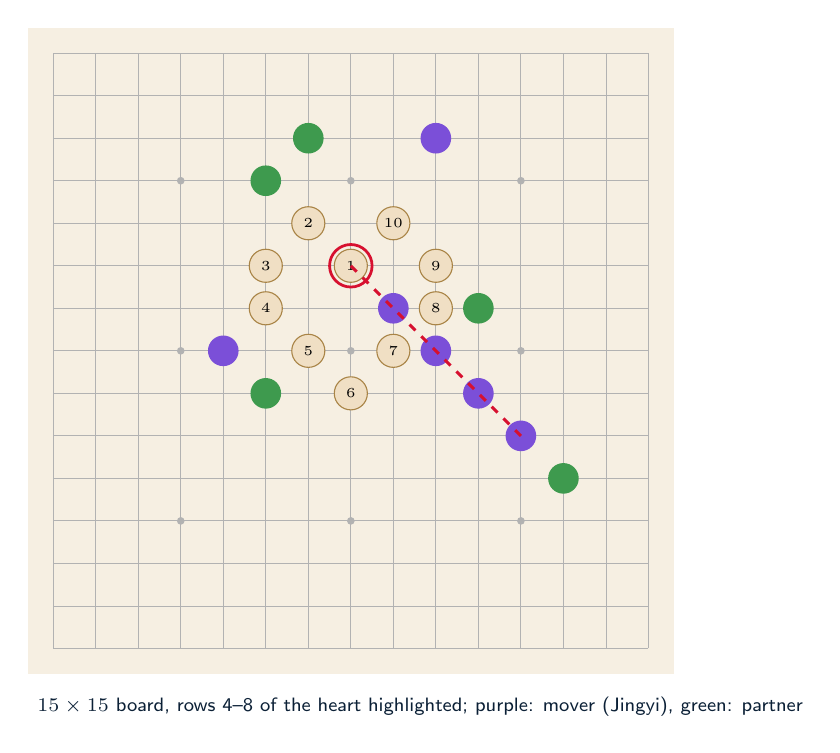
\begin{tikzpicture}[x=5.4mm, y=5.4mm, hpt/.style={circle, draw=gold!80!black, fill=gold!35, inner sep=0pt, minimum size=4.2mm, font=\scriptsize}]
    \fill[cream] (-0.6,-0.6) rectangle (14.6,14.6);
    \draw[gray!60, line width=0.3pt, step=1] (0,0) grid (14,14);
    \foreach \i in {3,7,11} \foreach \j in {3,7,11} \fill[gray!60] (\i,\j) circle (0.09);
    \node[hpt] at (7,9) {\tiny 1};
    \node[hpt] at (6,10) {\tiny 2};
    \node[hpt] at (5,9) {\tiny 3};
    \node[hpt] at (5,8) {\tiny 4};
    \node[hpt] at (6,7) {\tiny 5};
    \node[hpt] at (7,6) {\tiny 6};
    \node[hpt] at (8,7) {\tiny 7};
    \node[hpt] at (9,8) {\tiny 8};
    \node[hpt] at (9,9) {\tiny 9};
    \node[hpt] at (8,10) {\tiny 10};
    \fill[ygreen] (12,4) circle (0.36); \fill[ygreen] (5,11) circle (0.36); \fill[ygreen] (6,12) circle (0.36); \fill[ygreen] (10,8) circle (0.36); \fill[ygreen] (5,6) circle (0.36);
    \fill[jpurple] (8,8) circle (0.36); \fill[jpurple] (9,7) circle (0.36); \fill[jpurple] (10,6) circle (0.36); \fill[jpurple] (11,5) circle (0.36); \fill[jpurple] (4,7) circle (0.36); \fill[jpurple] (9,12) circle (0.36);
    \draw[merred, line width=1.1pt, dashed] (7,9) -- (11,5);
    \draw[merred, line width=1pt] (7,9) circle (0.5);
    \node[anchor=north west, font=\scriptsize\sffamily, text=navy] at (-0.6,-0.9) {$15\times15$ board, rows 4--8 of the heart highlighted; purple: mover (Jingyi), green: partner};
  \end{tikzpicture}
  \caption{Ten answers draw a heart. The gold discs are the ten cells of $\mathcal{H}$ in the order they
  are found (Eq.~\ref{eq:win}); the stones are position~1 as generated in the source
  (\code{heart-1}): six purple stones for the mover, five green decoys, and the unique winning cell
  (red ring) completing a diagonal five. Later positions are built the same way around the other nine
  cells, so solved answers accumulate into the outline.}
  \Description{A Gomoku grid with ten numbered gold discs forming a heart, a few purple and green stones, and a red ring marking the winning cell on a dashed diagonal.}
  \label{fig:heart}
\end{figure}

\paragraph{6. Our Songs.} Six songs the couple share (among them \zh{只对你有感觉} and
\zh{天下第一好}) play a passage through the official embedded players: QQ Music for the player in
China and YouTube for the player in the United States, each switchable. The site hosts no audio.
Embedded players expose no playback events, so the options unlock after eight seconds on screen,
whether or not the passage was heard.

\paragraph{7. Libra and Scorpius.} Yifan is a Libra (25 September) and Jingyi a Scorpio
(31 October); in the sky the two constellations are neighbours, and Libra's two brightest stars
still bear the Arabic names of the Scorpion's claws, \emph{Zubenelgenubi} and
\emph{Zubeneschamali}. The level projects 21 manually entered stars, six for Libra and fifteen for Scorpius,
and asks the player to draw 20 edges. The source records coordinates as J2000 right ascension
and declination, following the conventions in Meeus~\cite{meeus1998astronomical}; the chart is an
illustration, not a view of either player's current night sky.

\paragraph{8. Us, in Old Verse.} Five classical lines about love lose their second half, to be
restored from a bank of characters: a farewell traditionally attributed to Su Wu, \kai{结发为夫妻，恩爱两不疑};
Guan Daosheng's \emph{Song of You and Me}; a couplet of Li Shangyin; the paired birds of the
sixth-century anthology \emph{New Songs from a Jade Terrace}~\cite{birrell1982jade}; and an
anonymous couplet. Each solved line shows a plain English gloss.

\paragraph{9. Meridian.} The last level is a pair of rings, called \emph{Meridian}, modelled
procedurally in Blender from a Python script (Figure~\ref{fig:ring}). The pair share a signature:
a yellow-gold line inlaid around a platinum band like a meridian on a globe, a hidden sapphire
inside the bottom, and an inner engraving that carries the \emph{other} person's name and birthday,
the date they met and the coordinates of the airport where they will meet ($40.64^\circ$N
$73.78^\circ$W). Her ring exists in two designs, a solitaire on four compass prongs (v1) and the
current flush-set stone sunk into his band's profile (v2); the page keeps both as a design history.
The level is cleared only one way: the player tries the ring on through the camera and takes a
photo (Section~\ref{sec:sensing}).

\begin{figure}[t]
  \centering
  \includegraphics[width=0.325\columnwidth]{figures/hers_v1_hero.jpg}\hfill
  \includegraphics[width=0.325\columnwidth]{figures/hers_hero.jpg}\hfill
  \includegraphics[width=0.325\columnwidth]{figures/his_hero.jpg}
  \caption{The Meridian pair, path-traced from the procedural Blender model: hers v1 (solitaire,
  halo and graduated shoulder stones), hers v2 (flush-set 4.2\,mm stone in a 5\,mm flat band), and
  his (brushed flat comfort-fit band). The gold meridian runs around each band.}
  \Description{Three renders of rings on a dark background: a diamond solitaire, a flat band with
  a sunken stone, and a plain wide band, each with a thin gold line around it.}
  \label{fig:ring}
\end{figure}

\subsection{Two Days}\label{sec:days}
Two signposts lead from the square to a day in each city (Figure~\ref{fig:days}). Each is a second
map with the person's stops: Yifan's home, gym, his advisor's office, the golf course and the
pool in College Station; Jingyi's home with the cats at the door, her drive, the office and
Shenzhen Bay. Each stop has hours, and the person's sprite stands wherever the clock in their own
city puts them. A partner who opens Yifan's day at 9:49 p.m. in Shenzhen finds him at 8:49 a.m. at
his advisor's office. The schedules are authored, not sensed; they began as guesses and were corrected by the designer: Yifan drives
rather than taking the bus; Jingyi drives a Tesla rather than taking the metro; and the
Shenzhen Bay stop keeps a joke between them about where they will one day live.

\begin{figure}[t]
  \centering
  \begin{subfigure}[b]{0.49\columnwidth}\includegraphics[width=\linewidth]{figures/page-cs.jpg}\caption{A day of Yifan's}\end{subfigure}\hfill
  \begin{subfigure}[b]{0.49\columnwidth}\includegraphics[width=\linewidth]{figures/page-sz.jpg}\caption{A day of Jingyi's}\end{subfigure}
  \caption{The two cities as maps. The person stands at the stop whose hours contain the current
  local time in their own city: (a) Yifan at his advisor's office at 8:49 a.m.\ in College
  Station; (b) Jingyi at home at 9:49 p.m.\ in Shenzhen, the same instant.}
  \Description{Two pixel maps with roads and buildings, each with a person card above it and a row
  of stop buttons.}
  \label{fig:days}
\end{figure}

\subsection{Prologue and Finale}
Two cutscenes frame the game (Figure~\ref{fig:cutscenes}). They run in a small pixel theatre: a
$128\times80$ canvas scaled without smoothing, actors built from the town's sprite sheets, a
darkness layer with candle-like glows, particles, a synthesised score, and a caption box for words
and buttons.

\emph{The birthday prologue} plays once per player before the town opens. In College Station it is
9:47 a.m.; in Shenzhen 10:47 p.m., 73 minutes before Jingyi's birthday. Yifan, in a chef's hat,
bakes the cake against the Shenzhen clock. The player helps by whisking the batter (twelve taps),
placing ten strawberries in the same heart that the Gomoku answers make, and watching nine candles
lit (nine levels; in Chinese \zh{九} ``nine'' sounds like \zh{久} ``for a long time''). At the prologue's scripted Shenzhen midnight the lights go out, the door opens on the town (``In Yi Town there is no thirteen-hour
time difference''), everyone sings, the player makes a wish and blows the candles out, by
breathing into the microphone or holding a button.

\emph{The wedding} opens after the last letter, once both players have cleared the last level.
In the fountain garden at dusk, Rayford reveals why he had worn a suit all along: he is the
master of ceremonies. The groom waits under the arch, the bride walks the aisle to Mendelssohn's
\emph{Wedding March}, the scripted sequence asks for both characters' ``I do'' responses, with speech
recognition where supported, Coffee carries the rings down the aisle on a red pillow, the Meridian rings turn in
3D, and the scene ends in a kiss, bells, doves and a certificate to keep
(Figure~\ref{fig:cert}). Afterwards the town dresses the two sprites as bride and groom.

\begin{figure*}[t]
  \centering
  \includegraphics[width=0.245\textwidth]{figures/bday-03.jpg}\hfill
  \includegraphics[width=0.245\textwidth]{figures/bday-09.jpg}\hfill
  \includegraphics[width=0.245\textwidth]{figures/bday-27.jpg}\hfill
  \includegraphics[width=0.245\textwidth]{figures/bday-37.jpg}\\[3pt]
  \includegraphics[width=0.245\textwidth]{figures/wed-03.jpg}\hfill
  \includegraphics[width=0.245\textwidth]{figures/wed-11.jpg}\hfill
  \includegraphics[width=0.245\textwidth]{figures/wed-21.jpg}\hfill
  \includegraphics[width=0.245\textwidth]{figures/wed-23.jpg}
  \caption{The two cutscenes, left to right. Top, the birthday prologue: the kitchen at 9:47 a.m.\
  in College Station (10:47 p.m.\ in Shenzhen) with both clocks on the wall; whisking the batter;
  nine candles on the finished cake; singing at Shenzhen midnight with the cats. Bottom, the
  wedding: the guests take their seats; the bride walks the aisle; Coffee brings the rings; the
  Meridian rings in 3D over the ceremony.}
  \Description{Eight pixel-art frames. Top row: a pink kitchen, a chef at a table, a cake with
  candles, the same kitchen dark with candlelight. Bottom row: a garden with a flower arch at sunset,
  a couple under the arch, a cat carrying a pillow, two large 3D rings in circles.}
  \label{fig:cutscenes}
\end{figure*}

\begin{figure}[t]
  \centering
  \includegraphics[width=0.78\columnwidth]{figures/wed-cert.jpg}
  \caption{The certificate at the end of the wedding, saved as an image through the phone's share
  sheet. It records the day of the ceremony, the day they met and the day they will meet.}
  \Description{A cream certificate card with two cartoon avatars and the names Yifan Yang and Jingyi Chen joined by a heart, on confetti.}
  \label{fig:cert}
\end{figure}

%% ===================================================================================
\section{After the Town}\label{sec:after}
The first version described a finished gift with a beginning and an end. In the four weeks that
followed, the dashboard gained four cards (Figure~\ref{fig:cards}). Three are products kept in
the same repository and described here; the fifth card links to a separate project of the
couple's and is not discussed. None of the three is a level. None has a lock, none counts toward
progress, and nothing in them waits to be revealed, so staged access (\dc{2}) and delayed
disclosure (\dc{6}) do not apply to them. Table~\ref{tab:after} sets them against the
commitments.

\begin{figure}[t]
  \centering
  \begin{subfigure}[b]{0.325\columnwidth}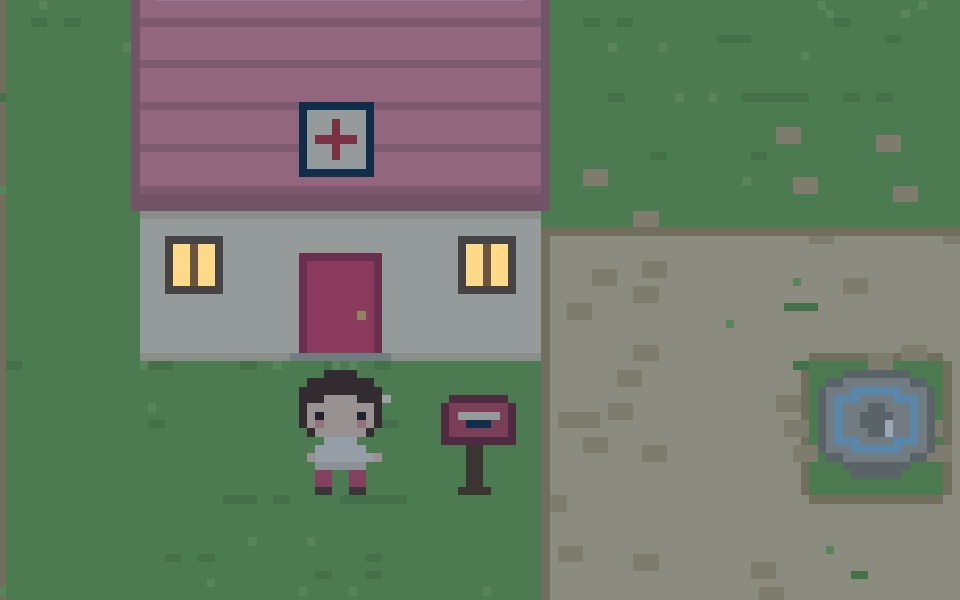
\includegraphics[width=\linewidth]{figures/card-clinic.jpg}\caption{Infirmary}\end{subfigure}\hfill
  \begin{subfigure}[b]{0.325\columnwidth}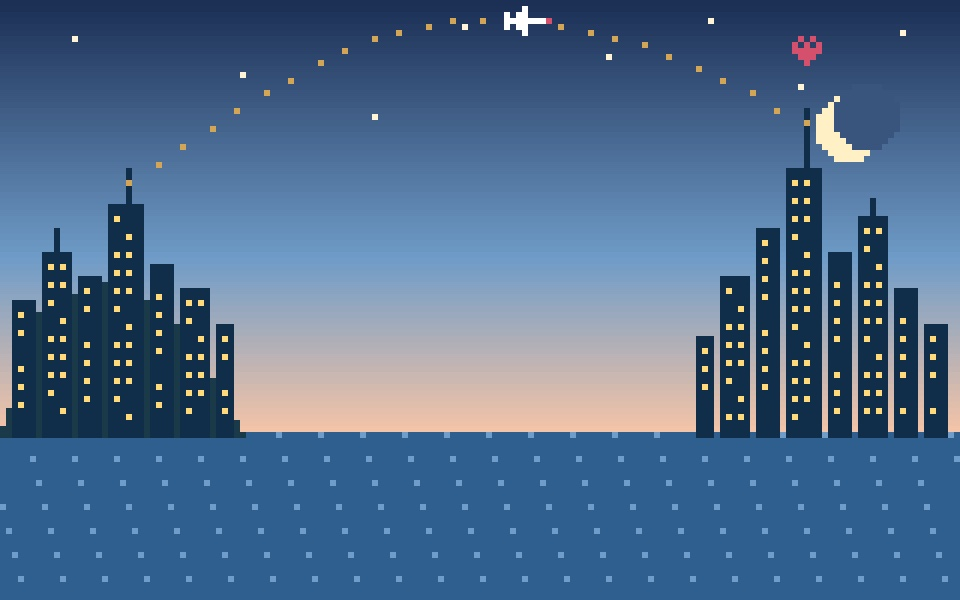
\includegraphics[width=\linewidth]{figures/card-trip.jpg}\caption{Trip}\end{subfigure}\hfill
  \begin{subfigure}[b]{0.325\columnwidth}
\includegraphics[width=\linewidth]{figures/card-ask.jpg}\caption{Request box}\end{subfigure}\\[3pt]
  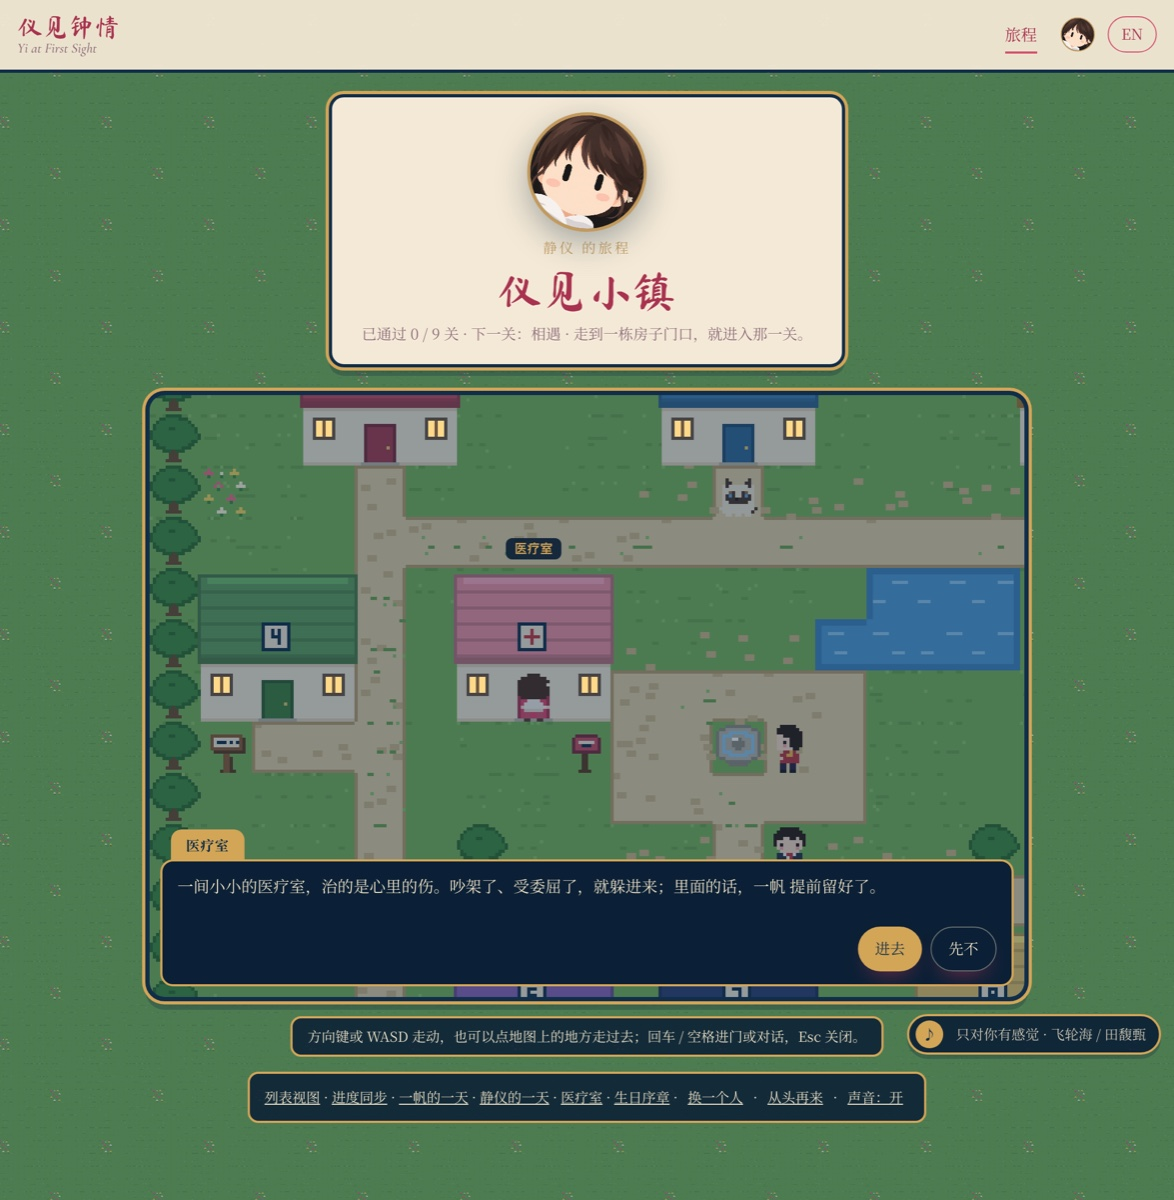
\includegraphics[width=0.9\columnwidth]{figures/clinic-town.jpg}
  \caption{After the town. Top: the pictures on three of the dashboard's cards, each drawn by a
  script in the repository. Bottom: the infirmary as a house in the town, north-west of the
  fountain, with the talk box that opens at its door. It has no number on its roof and no cat at
  its door.}
  \Description{Three small pixel pictures: a pink house with a red cross, two cities joined by a
  dotted route with a plane, and an envelope sealed with a heart. Below, a screenshot of the pixel
  town with a pink-roofed house marked by a cross and a dialogue box in Chinese.}
  \label{fig:cards}
\end{figure}

\begin{table}[t]
  \caption{The three later products against the commitments written for the town.
  \emph{kept}: the product follows it; \emph{n/a}: nothing in the product for it to govern;
  \emph{broken}: the product departs from it by design.}
  \label{tab:after}
  \small
  \begin{tabular}{@{}p{0.34\columnwidth}ccc@{}}
    \toprule
    Commitment & Infirmary & Trip & Request box \\
    \midrule
    \dc{1} Memory-derived mechanics & kept & n/a & n/a \\
    \dc{2} Staged access & n/a & n/a & n/a \\
    \dc{3} Local state, no backend & kept & kept & broken \\
    \dc{4} Bilingual coverage & kept & kept & kept \\
    \dc{5} Drawn in code & kept & kept & kept \\
    \dc{6} Delayed disclosure & n/a & n/a & n/a \\
    \bottomrule
  \end{tabular}
\end{table}

\subsection{The Infirmary}
On 3 November the recipient said, as the changelog records it,
``\zh{以后我受伤了我就不跟你说话了，我就躲进去}'' (``from now on, when I am hurt I will not talk to
you; I will hide in there''). The infirmary was added the next day (\code{397db28}) as a pink
house by the square and as the second card. A visitor says what hurts, choosing among a quarrel,
a hurt, missing the other without wanting to speak first, and plain tiredness. Three slow
breaths follow, which can be skipped. Then the page shows a letter that the other partner wrote
in advance for that hurt. A cabinet gives one-line notes at random, and a chart takes private
lines that stay in the browser's local storage.

Two details carry the design. The letter opens with what its writer is doing at that moment,
computed from the clock in the writer's city and an authored schedule, for example that it is
past three in the morning there and he is asleep. The same caveat applies as to the city days in
Section~\ref{sec:days}: this is a schedule, not sensed presence. And leaving offers one button,
``tell them I am out'', which hands the phone's share sheet a single line with the length of the
visit. Nothing is sent without that tap, and the dashboard card shows no count of visits, because
how often someone has hidden is theirs alone.

The authorship of the letters needs stating exactly. There are four letters and eighteen notes
for each partner. Both sets were first written on 4 November as drafts ``in each one's voice, for
each to rewrite'' (\code{73e54bc}). By the cut-off the record shows one of Yifan's letters
replaced with his own text (\code{dc62d23}) and no revision of the set attributed to Jingyi. The
words the infirmary shows a visitor as hers are therefore, on the record, words written for her.

\subsection{See You in New York}
The first version's countdown pointed at a symbolic ticket, hand-drawn during a video call. On
8 November Jingyi booked her flights, and the site followed (\code{d9de84b}): the countdown and
the gold line on the Love Map now end at her landing on 4 February 2027, and the page for the
trip shows both legs as boarding passes with local times. Its clock knows five phases: before
departure, in the air, together, flying home, and home. During the stay it counts ``day $n$ of
11''. Below it is an itinerary with one row for each day, to be written and photographed as the
days happen; an unwritten day reads ``still growing''. The hand-drawn ticket stays in the game as
a memory, in the Moments level and the first level's quiz. The page asks for no player, since it
has no progress to keep.

\subsection{Ask Yifan}
The fourth card opens a composer like that of a chat application: a text box, a paperclip, drag
and drop, and paste for screenshots (\code{ea2c088}, 24 November). Jingyi writes what she needs
help with, attaches up to ten files and 18\,MB, and sends. Her request reaches Yifan's inbox as
one email with the files attached. What she sent stays on her device as bubbles marked sending,
sent or failed; a failed send keeps its text and files and offers to try again. The specification
describes the page as one-way on purpose: the answer was to come over the couple's usual
messaging, or as the thing done.

A browser cannot send an email with attachments, so this product required the site's first
server-side code, and within a day it acquired an automated answerer. Both are described in
Section~\ref{sec:askpath}. We say nothing in this paper about what her requests ask for.

%% ===================================================================================
\section{System}\label{sec:system}

\subsection{Architecture}
\yt{} is a static single-page application in strict TypeScript, built with Vite and served from
static hosting under the couple's domain (Figure~\ref{fig:arch}). The deployment configuration
targets GitHub Pages. There is no author-operated backend for progress; since version 1.22 there
is one for requests (Section~\ref{sec:askpath}), which Figure~\ref{fig:arch} does not show. Each feature
is a folder (\code{src/features/<name>/}) with its page module, styles, data, tests and a README,
and each page is a function \code{render(root) $\Rightarrow$ cleanup} loaded lazily by a path
router, so the main bundle carries only the shell and the town. Heavy modules (Leaflet for the map,
three.js for the ring, MediaPipe for the try-on) load only inside the level that needs them. A
service worker precaches the shell and caches eligible media after retrieval. The cached
town can run offline, but remote song embeds and browser-dependent speech recognition are not
guaranteed offline; cache eviction and previously unfetched assets also limit availability.

\begin{figure}[t]
  \centering
  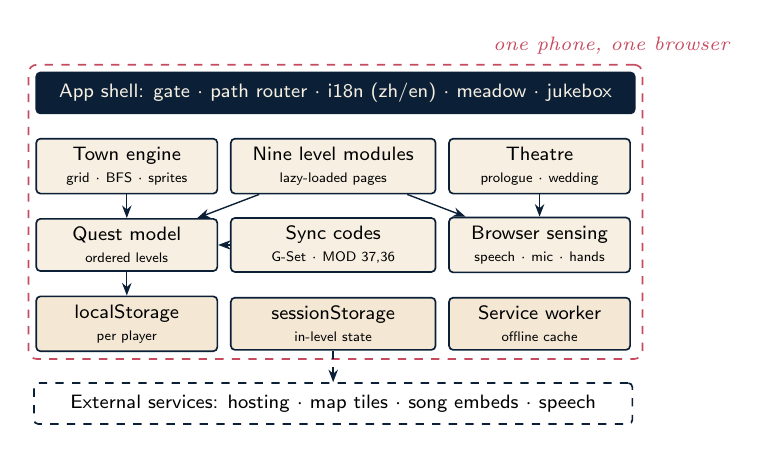
\begin{tikzpicture}[
      font=\scriptsize\sffamily,
      box/.style={draw=navy, line width=0.6pt, fill=cream, rounded corners=1.5pt, align=center, inner sep=3pt, minimum height=5.2mm},
      store/.style={box, fill=gold!25},
      ext/.style={box, dashed, fill=white},
      arr/.style={-{Stealth[length=1.6mm]}, navy, line width=0.5pt}]
    \node[box, minimum width=7.6cm, fill=navy, text=cream] (shell) {App shell: gate $\cdot$ path router $\cdot$ i18n (zh/en) $\cdot$ meadow $\cdot$ jukebox};
    \node[box, below=3mm of shell.south west, anchor=north west, minimum width=2.3cm] (town) {Town engine\\\tiny grid $\cdot$ BFS $\cdot$ sprites};
    \node[box, right=1.5mm of town, minimum width=2.6cm] (levels) {Nine level modules\\\tiny lazy-loaded pages};
    \node[box, right=1.5mm of levels, minimum width=2.3cm] (theatre) {Theatre\\\tiny prologue $\cdot$ wedding};
    \node[box, below=3mm of town, minimum width=2.3cm] (quest) {Quest model\\\tiny ordered levels};
    \node[box, right=1.5mm of quest, minimum width=2.6cm] (sync) {Sync codes\\\tiny G-Set $\cdot$ MOD 37,36};
    \node[box, right=1.5mm of sync, minimum width=2.3cm] (sense) {Browser sensing\\\tiny speech $\cdot$ mic $\cdot$ hands};
    \node[store, below=3mm of quest, minimum width=2.3cm] (ls) {localStorage\\\tiny per player};
    \node[store, right=1.5mm of ls, minimum width=2.6cm] (ss) {sessionStorage\\\tiny in-level state};
    \node[store, right=1.5mm of ss, minimum width=2.3cm] (sw) {Service worker\\\tiny offline cache};
    \node[ext, below=4mm of ss, minimum width=7.6cm] (ext) {External services: hosting $\cdot$ map tiles $\cdot$ song embeds $\cdot$ speech};
    \node[draw=rose, dashed, rounded corners=3pt, line width=0.6pt, fit=(shell)(ls)(sw), inner sep=2.5pt,
          label={[rose, font=\scriptsize\itshape]above right:one phone, one browser}] {};
    \draw[arr] (town) -- (quest); \draw[arr] (levels) -- (quest); \draw[arr] (levels) -- (sense);
    \draw[arr] (theatre) -- (sense); \draw[arr] (quest) -- (ls); \draw[arr] (sync) -- (quest);
    \draw[arr, dashed] (ss.south) -- (ext.north);
  \end{tikzpicture}
  \caption{Architecture of application modules and local state. The dashed boundary marks browser
  components, not a confidentiality boundary: static assets are hosted remotely, external requests
  expose request metadata, and speech recognition may use a remote service. Progress crosses
  devices through a manually exchanged code.}
  \Description{A block diagram: an app shell above three modules, which depend on a quest model,
  sync codes and browser sensing, which sit above three storage layers, all inside a dashed boundary
  labelled one phone, one browser; a dashed box below for external hosting, map, media and speech services.}
  \label{fig:arch}
\end{figure}

\subsection{The Quest Model}
Let $L = (\ell_1,\dots,\ell_9)$ be the ordered level registry and $C_p \subseteq L$ the set of
levels player $p$ has cleared on a device. A level is unlocked iff it is first or its predecessor
is cleared:
\begin{equation}\label{eq:unlock}
  \mathrm{unlocked}_p(\ell_i) \iff i = 1 \;\lor\; \ell_{i-1} \in C_p .
\end{equation}
Clearing adds to $C_p$ and nothing ever removes from it, except an explicit reset. The next level
to play is the first one not yet cleared, $\mathrm{current}(p) = \ell_{\min\{i : \ell_i \notin C_p\}}$.
The router enforces the lock, and a second guard requires that a level be entered through its door:
walking onto the door sets a one-shot token $\tau$ in \code{sessionStorage}, and a level route
without the token redirects to the town, so that
\begin{equation}\label{eq:enter}
  \mathrm{enter}_p(\ell_i) \iff \mathrm{unlocked}_p(\ell_i) \;\land\; \tau = \mathrm{route}(\ell_i) .
\end{equation}
Figure~\ref{fig:chain} shows the whole sequence, including the two scenes gated on both players. Level numbers are derived from the registry, so inserting a level (the
Poems level was inserted before the last one during development) renumbers every house, sign and
string at once; a test fails until the new house has a door that the town's path search can reach.

\begin{figure}[t]
  \centering
  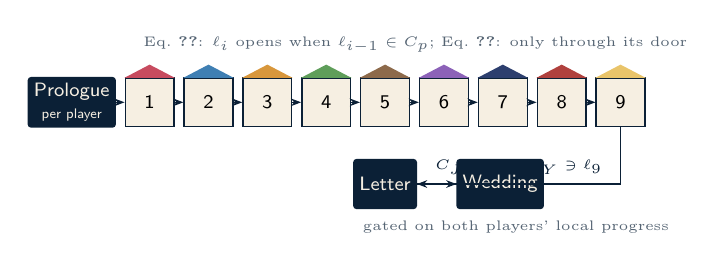
\begin{tikzpicture}[font=\scriptsize\sffamily, node distance=1.1mm,
      lv/.style={draw=navy, line width=0.5pt, fill=cream, minimum width=6.2mm, minimum height=6.2mm, inner sep=0pt},
      scene/.style={draw=navy, line width=0.5pt, fill=navy, text=cream, rounded corners=1pt, minimum height=6.2mm, inner sep=2pt, align=center},
      arr/.style={-{Stealth[length=1.3mm]}, navy, line width=0.45pt}]
    \node[scene] (pro) {Prologue\\\tiny per player};
    \definecolor{roof1}{HTML}{C74B5F}
    \node[lv, right=of pro] (l1) {1};
    \fill[roof1] ([yshift=-0.2pt]l1.north west) -- ([yshift=1.6mm]l1.north) -- ([yshift=-0.2pt]l1.north east) -- cycle;
    \draw[arr] (pro) -- (l1);
    \definecolor{roof2}{HTML}{3F7FB3}
    \node[lv, right=of l1] (l2) {2};
    \fill[roof2] ([yshift=-0.2pt]l2.north west) -- ([yshift=1.6mm]l2.north) -- ([yshift=-0.2pt]l2.north east) -- cycle;
    \draw[arr] (l1) -- (l2);
    \definecolor{roof3}{HTML}{D8973C}
    \node[lv, right=of l2] (l3) {3};
    \fill[roof3] ([yshift=-0.2pt]l3.north west) -- ([yshift=1.6mm]l3.north) -- ([yshift=-0.2pt]l3.north east) -- cycle;
    \draw[arr] (l2) -- (l3);
    \definecolor{roof4}{HTML}{5F9E5A}
    \node[lv, right=of l3] (l4) {4};
    \fill[roof4] ([yshift=-0.2pt]l4.north west) -- ([yshift=1.6mm]l4.north) -- ([yshift=-0.2pt]l4.north east) -- cycle;
    \draw[arr] (l3) -- (l4);
    \definecolor{roof5}{HTML}{8D6A4B}
    \node[lv, right=of l4] (l5) {5};
    \fill[roof5] ([yshift=-0.2pt]l5.north west) -- ([yshift=1.6mm]l5.north) -- ([yshift=-0.2pt]l5.north east) -- cycle;
    \draw[arr] (l4) -- (l5);
    \definecolor{roof6}{HTML}{8C62B8}
    \node[lv, right=of l5] (l6) {6};
    \fill[roof6] ([yshift=-0.2pt]l6.north west) -- ([yshift=1.6mm]l6.north) -- ([yshift=-0.2pt]l6.north east) -- cycle;
    \draw[arr] (l5) -- (l6);
    \definecolor{roof7}{HTML}{2D3F6E}
    \node[lv, right=of l6] (l7) {7};
    \fill[roof7] ([yshift=-0.2pt]l7.north west) -- ([yshift=1.6mm]l7.north) -- ([yshift=-0.2pt]l7.north east) -- cycle;
    \draw[arr] (l6) -- (l7);
    \definecolor{roof8}{HTML}{B0413E}
    \node[lv, right=of l7] (l8) {8};
    \fill[roof8] ([yshift=-0.2pt]l8.north west) -- ([yshift=1.6mm]l8.north) -- ([yshift=-0.2pt]l8.north east) -- cycle;
    \draw[arr] (l7) -- (l8);
    \definecolor{roof9}{HTML}{E9C46A}
    \node[lv, right=of l8] (l9) {9};
    \fill[roof9] ([yshift=-0.2pt]l9.north west) -- ([yshift=1.6mm]l9.north) -- ([yshift=-0.2pt]l9.north east) -- cycle;
    \draw[arr] (l8) -- (l9);
    \node[scene, below=4mm of l5] (let) {Letter};
    \node[scene, right=5mm of let] (wed) {Wedding};
    \draw[arr] (l9.south) |- node[pos=0.75, above, font=\tiny] {$C_J \ni \ell_9 \land C_Y \ni \ell_9$} (let.east);
    \draw[arr] (let) -- (wed);
    \node[below=0.3mm of let.south west, anchor=north west, font=\tiny, text=navy!70] {gated on both players' local progress};
    \node[above=1.8mm of l1.north, anchor=south west, font=\tiny, text=navy!70, xshift=-2mm] {Eq.~\ref{eq:unlock}: $\ell_i$ opens when $\ell_{i-1} \in C_p$; Eq.~\ref{eq:enter}: only through its door};
  \end{tikzpicture}
  \caption{The sequence of play. Nine houses open in order per player; the letter and the wedding
  open only when both players' completion sets on the device contain the last level.}
  \Description{A chain of nine numbered boxes with coloured roofs following a prologue box, and a branch from box nine down to letter and wedding boxes.}
  \label{fig:chain}
\end{figure}

\subsection{Progress without a Server}
Each phone holds its own $C_p$. Because $C_p$ only grows, it is a grow-only set (G-Set), the
simplest state-based CRDT~\cite{shapiro2011crdt}: the merge of two replicas is their union,
\begin{equation}\label{eq:merge}
  C_p \sqcup C'_p = C_p \cup C'_p ,
\end{equation}
which is commutative, associative and idempotent. Replicas converge if all updates are eventually exchanged, both phones use the same
level registry and no reset occurs. Repeated imports are idempotent; an old code cannot remove
completion flags, but incomplete exchange can leave the two views different. The
only channel needed is one the couple already use every day: a chat message.

\paragraph{Progress codes.} A code encodes one player and a bitmask of cleared levels,
written in base 36 after a player letter $\lambda_p \in \{\code{J}, \code{Y}\}$ and followed by one
check character $\chi$ (Figure~\ref{fig:sync}):
\begin{equation}\label{eq:code}
  m = \sum_{\ell_i \in C_p} 2^{\,i-1}, \qquad
  \mathrm{code}(p, C_p) = \lambda_p \,\Vert\, \beta_{36}(m) \,\Vert\, \chi\big(\lambda_p \Vert \beta_{36}(m)\big),
\end{equation}
where $\Vert$ is concatenation and $\beta_{36}$ writes a number in base 36. The decoder accepts a
string only if its last character equals $\chi$ of the rest, its first is a player letter and
$0 \le m < 2^{9}$. With nine levels $m \le 511 = \mathrm{E7}_{36}$, so a
code is at most four characters: \code{JVA} says that Jingyi has cleared $m = 31$, the first five
levels (Table~\ref{tab:codes}). The check character follows the hybrid system ISO~7064
MOD~37,36~\cite{iso7064}. Writing $a_j \in \{0,\dots,35\}$ for the value of the $j$-th body
character and starting from $p_0 = 36$,
\begin{equation}\label{eq:check}
  s_j = \big((p_{j-1} + a_j) \bmod 36\big) \text{ or } 36 \text{ if } 0, \qquad
  p_j = 2 s_j \bmod 37 ,
\end{equation}
and the check character is the symbol of value $(37 - p_n) \bmod 36$. We checked the scheme exhaustively over all
1{,}024 valid codes: 140{,}840 single-character substitutions and 2{,}943 transpositions of two
different adjacent characters. It rejects every substitution. Of the transpositions it rejects
all but five. One of those (\code{JI0}$\to$\code{IJ0}) is still refused because \code{I} is not a
player letter. The other four all swap a \code{0} and a \code{1} inside the mask
(\code{J801}$\leftrightarrow$\code{J810}, \code{YE01}$\leftrightarrow$\code{YE10}): the rule above
maps a running sum of 0 to 36, so a zero digit and its neighbour can trade places unseen.
An accepted typo may add unearned completion flags and unlock later content, including the finale. An earlier version used a plain weighted sum,
which let some one-character typos through; it was later replaced, invalidating older
codes. Codes are not authenticated: a person can construct completion for either player. They
carry no schema version, so registry insertions or reordering can reinterpret bits. Reset is outside
the grow-only model; importing an earlier code after reset restores its flags. A code may also
travel in a link (\code{/sync?c=JVA}), exposing its payload to the hosting request and potentially
to browser history or the channel through which it is sent.

\begin{table}[t]
  \caption{Example progress codes: player letter, base-36 mask (Eq.~\ref{eq:code}) and the check character of Eq.~\ref{eq:check}.}
  \label{tab:codes}
  \small
  \begin{tabular}{@{}lrll@{}}
    \toprule
    Cleared & Mask $m$ & Base 36 & Code \\
    \midrule
    Jingyi, levels 1--5 & 31 & \code{V} & \code{JVA} \\
    Jingyi, all nine & 511 & \code{E7} & \code{JE7Z} \\
    Yifan, all nine & 511 & \code{E7} & \code{YE7O} \\
    Yifan, none & 0 & \code{0} & \code{Y0C} \\
    \bottomrule
  \end{tabular}

\end{table}

\begin{figure}[t]
  \centering
  \begin{tikzpicture}[font=\scriptsize\sffamily,
      phone/.style={draw=navy, line width=0.6pt, rounded corners=2mm, fill=cream, minimum width=24mm, minimum height=26mm},
      chip/.style={draw=navy!60, fill=white, rounded corners=0.6pt, inner sep=1.5pt, font=\scriptsize\ttfamily},
      arr/.style={-{Stealth[length=1.4mm]}, navy, line width=0.5pt}]
    \node[phone] (a) at (0,0) {};
    \node[phone] (b) at (5.4,0) {};
    \node[anchor=north, text=navy] at ([yshift=-1.2mm]a.north) {Jingyi's phone};
    \node[anchor=north, text=navy] at ([yshift=-1.2mm]b.north) {Yifan's phone};
    \node[anchor=north, align=center] at ([yshift=-6mm]a.north) {$C_J = \{\ell_1,\dots,\ell_5\}$\\$C_Y = \{\ell_1, \ell_2\}$};
    \node[anchor=north, align=center] at ([yshift=-6mm]b.north) {$C_J = \{\ell_1, \ell_2, \ell_3\}$\\$C_Y = \{\ell_1,\dots,\ell_7\}$};
    \node[anchor=south, align=center, text=merred] at ([yshift=1.2mm]a.south) {after import:\\$C_Y = \{\ell_1,\dots,\ell_7\}$};
    \node[anchor=south, align=center, text=merred] at ([yshift=1.2mm]b.south) {after import:\\$C_J = \{\ell_1,\dots,\ell_5\}$};
    \draw[arr] ([yshift=3mm]a.east) -- node[above, chip] {JVA} node[below, font=\tiny] {chat message} ([yshift=3mm]b.west);
    \draw[arr] ([yshift=-3mm]b.west) -- node[above, chip] {Y3J} node[below, font=\tiny] {or a link \code{/sync?c=Y3J}} ([yshift=-3mm]a.east);
    \node[below=1.5mm of a.south west, anchor=north west, font=\scriptsize] (lay) {
      \begin{tikzpicture}[font=\scriptsize\ttfamily, every node/.style={draw=navy, fill=white, minimum height=5mm, inner sep=2pt}]
        \node (p) {J}; \node[right=0pt of p, fill=gold!30] (m) {V}; \node[right=0pt of m] (c) {A};
        \node[draw=none, fill=none, below=0.3mm of p, font=\tiny\sffamily] {$\lambda_p$};
        \node[draw=none, fill=none, below=0.3mm of m, font=\tiny\sffamily] {$\beta_{36}(31)$};
        \node[draw=none, fill=none, below=0.3mm of c, font=\tiny\sffamily] {$\chi$};
      \end{tikzpicture}};
    \node[right=2mm of lay, anchor=west, font=\scriptsize\sffamily, align=left, text=navy] {$m = 31 = 000011111_2$: bit $i$ is set when $\ell_i \in C_J$\\union merge (Eq.~\ref{eq:merge}) never removes a level and\\converges once both codes have travelled};
  \end{tikzpicture}
  \caption{Progress without a server. Each phone keeps both players' completion sets; a short code
  (Eq.~\ref{eq:code}) carries one set across in a chat message or a link, and the receiver takes the
  union (Eq.~\ref{eq:merge}). Below: the three fields of \code{JVA}.}
  \Description{Two phone outlines with sets of levels inside, two arrows between them labelled with three-letter codes, and a three-cell diagram of a code's fields below.}
  \label{fig:sync}
\end{figure}

\paragraph{Three layers of storage.} Cleared levels live in \code{localStorage} under a key per
player; half-finished state inside a level (the Gomoku position reached, the stars joined so far)
lives in \code{sessionStorage}, so a reload or a language switch inside a level does not restart it,
and it is dropped when the level is cleared; and a service worker keeps the site itself. When the
browser blocks storage, an in-memory store keeps progress for the visit.

\subsection{The Town Engine}
The town is a grid of characters (\code{.}\ grass, \code{\#} path, \code{\textasciitilde}\ water,
\code{T} tree, \code{O} fountain, and so on). Movement is one tile per 190\,ms with an ease-out
interpolation $e(t) = 1 - (1-t)^2$ of the step's progress $t \in [0,1]$; the pure functions \code{step} and \code{faced} decide movement and facing and are
unit-tested, while a class wires them to a canvas and one animation loop. A tap on the map runs a
breadth-first search over walkable tiles and queues the resulting steps. The camera follows the
player. The same engine takes any map, so the two cities reuse it with their own grids, roads and a
basketball court.

\paragraph{Art as text (\dc{5}).} A sprite is an array of strings, one character per pixel, and
a palette that maps characters to colours. A figure is a $12\times12$ body per facing over four
rows of legs shared between facings, so a walk cycle is the same two leg frames under different
bodies, and the side view is mirrored. Tiles (grass with flowers, paths that join their neighbours,
roofs in each level's colour, lit windows) are painted procedurally. The README banner, the favicon
and the app icons are generated from the same strings by scripts, so a new outfit appears
everywhere at once.

\paragraph{Daylight by city.} Let $h_p$ be the current hour in player $p$'s time zone
(\code{Asia/Shanghai} or \code{America/Chicago}). The phase of the sky and the person's place in a
city day are
\begin{equation}\label{eq:phase}
  \phi(h) = \begin{cases} \text{dawn} & 6 \le h < 7, \\ \text{day} & 7 \le h < 17, \\ \text{dusk} & 17 \le h < 19, \\ \text{night} & \text{otherwise,} \end{cases}
\end{equation}
\begin{equation}\label{eq:stop}
  \mathrm{stop}(h) = \min\big\{\, j : \exists\,[a,b) \in W_j,\; a \le h \bmod 24 < b \,\big\},
\end{equation}
where $W_j$ is the set of hour windows of the $j$-th stop. Dawn, dusk and night each lay a coloured
wash over the map (night: navy at 42\% opacity) and light the windows. Because $h_J$ and $h_Y$
differ by the two cities' offset, the same instant falls in different phases for the two players
(Figure~\ref{fig:bands}).

\begin{figure}[t]
  \centering
  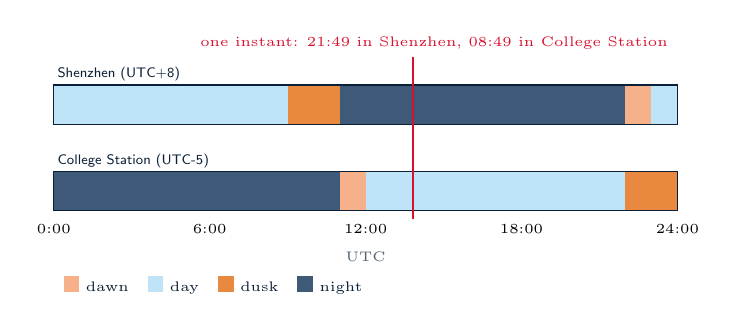
\begin{tikzpicture}[x=3.3mm, y=1mm, font=\scriptsize\sffamily]
    \definecolor{cday}{HTML}{BFE3F7}\definecolor{cdawn}{HTML}{F6B18A}\definecolor{cdusk}{HTML}{E8893F}\definecolor{cnight}{HTML}{3E5A78}
    % bars span 24 h of UTC; Shenzhen is UTC+8, College Station UTC-5 (CDT, as during development)
    \foreach \name/\off/\yy in {Shenzhen (UTC+8)/8/11, College Station (UTC-5)/-5/0} {
      \foreach \u in {0,...,23} {
        \pgfmathtruncatemacro{\h}{mod(\u+\off+24,24)}
        \pgfmathsetmacro{\col}{(\h>=6 && \h<7) ? "cdawn" : ((\h>=7 && \h<17) ? "cday" : ((\h>=17 && \h<19) ? "cdusk" : "cnight"))}
        \fill[\col] (\u,\yy) rectangle (\u+1,\yy+5);
      }
      \draw[navy, line width=0.4pt] (0,\yy) rectangle (24,\yy+5);
      \node[anchor=south west, text=navy, font=\tiny\sffamily, inner sep=0.4mm] at (0,\yy+5) {\name};
    }
    \foreach \u in {0,6,12,18,24} \node[anchor=north, font=\tiny] at (\u,-0.5) {\u:00};
    \node[anchor=north, font=\tiny, text=navy!70] at (12,-4) {UTC};
    % the same instant: 13:49 UTC = 21:49 Shenzhen = 08:49 College Station
    \draw[merred, line width=0.9pt] (13.82,-1) -- (13.82,19.5);
    \node[anchor=south east, text=merred, font=\tiny] at (24,19.3) {one instant: 21:49 in Shenzhen, 08:49 in College Station};
    \node[anchor=north west, font=\tiny, text=navy] at (0,-7) {\tikz\fill[cdawn] (0,0) rectangle (2mm,2mm); dawn\quad \tikz\fill[cday] (0,0) rectangle (2mm,2mm); day\quad \tikz\fill[cdusk] (0,0) rectangle (2mm,2mm); dusk\quad \tikz\fill[cnight] (0,0) rectangle (2mm,2mm); night};
  \end{tikzpicture}
  \caption{The two skies over one UTC day (Eq.~\ref{eq:phase}), with the thirteen-hour offset in force
  during development. Night in one town overlaps day in the other for most of every day; the red line is
  the instant shown in Figure~\ref{fig:days}.}
  \Description{Two horizontal bars coloured by dawn, day, dusk and night phases, offset by thirteen hours, with a red vertical line marking one instant.}
  \label{fig:bands}
\end{figure}

\subsection{Sensing in the Browser}\label{sec:sensing}
Camera tracking and breath-amplitude processing run in application code on the device.
Browser speech recognition has a different processing boundary.

\emph{Voice.} The vow and the wedding's ``I do'' use the Web Speech API~\cite{w3c2023speech} in
Mandarin. The API allows a remote recognition service unless local processing is explicitly
required~\cite{w3c2023speech}, and the implementation does not require it, so voice samples may
leave the device. A typed fallback is available for the vow. Recognition alternatives are joined into one string $w$ and normalised
by $\nu$, which keeps only Han characters and Latin letters; with $\sqsubseteq$ for ``is a substring
of'' and $\mathcal{N}_p$ the accepted spellings of the partner's name,
\begin{align}
  \mathrm{vow}_p(w) \iff\;& \text{\zh{我爱你}} \sqsubseteq \nu(w) \;\land\; \text{\zh{我愿意}} \sqsubseteq \nu(w) \label{eq:vow} \\
  &\land\; \exists\, n \in \mathcal{N}_p :\ n \sqsubseteq \nu(w) . \nonumber
\end{align}

\emph{Breath.} Blowing out the candles reads the microphone with echo cancellation, noise
suppression and gain control off. For each frame $t$ of $N = 1{,}024$ samples $x_{t,i}$,
\begin{align}
  r_t &= \sqrt{\tfrac{1}{N}\textstyle\sum_{i=1}^{N} x_{t,i}^{2}}, \qquad
  s_t = 0.6\, s_{t-1} + 0.4 \min(1, 5 r_t), \label{eq:breath} \\
  \mathrm{blow}_t &\iff s_t > 0.32 . \nonumber
\end{align}
We rely on a breath being a loud, broadband rush on a phone microphone; the threshold was set by
hand and has not yet been calibrated across devices.

\emph{Hands.} The try-on runs MediaPipe's hand landmarker~\cite{lugaresi2019mediapipe,zhang2020hands}
on the camera stream, which returns 21 landmarks $\mathbf{k}_0, \dots, \mathbf{k}_{20}$ per hand
(Figure~\ref{fig:hand}). The ring's axis $\mathbf{a}$ follows the ring finger's proximal phalanx,
its ``up'' $\mathbf{u}$ is the back of the hand, taken from the palm normal $\mathbf{n}$ with the
sign given by the reported handedness, and its centre $\mathbf{c}$ sits a fraction $\beta = 0.38$
along the phalanx:
\begin{align}
  \mathbf{a} &= \frac{\mathbf{k}_{14} - \mathbf{k}_{13}}{\lVert \mathbf{k}_{14} - \mathbf{k}_{13} \rVert}, &
  \mathbf{n} &= \pm\,\frac{(\mathbf{k}_5 - \mathbf{k}_0) \times (\mathbf{k}_{17} - \mathbf{k}_0)}{\lVert (\mathbf{k}_5 - \mathbf{k}_0) \times (\mathbf{k}_{17} - \mathbf{k}_0) \rVert}, \label{eq:hand-axes} \\
  \mathbf{u} &= \frac{\mathbf{n} - (\mathbf{n}\cdot\mathbf{a})\,\mathbf{a}}{\lVert \mathbf{n} - (\mathbf{n}\cdot\mathbf{a})\,\mathbf{a} \rVert}, &
  \mathbf{c} &= (1-\beta)\,\mathbf{k}_{13} + \beta\,\mathbf{k}_{14}, \label{eq:hand-pose}
\end{align}
and the rotation is the orthonormal basis $R = [\,\mathbf{u} \times \mathbf{a},\ \mathbf{u},\ \mathbf{a}\,]$.
Scale comes from anatomy: the mean spacing of the middle, ring and little knuckles is the
ruler, set to a constant of 19.5\,mm (a working estimate for an adult hand),
\begin{equation}\label{eq:scale}
  \text{px/mm} = \tfrac{1}{2}\,\big(\lVert \mathbf{k}_9 - \mathbf{k}_{13}\rVert + \lVert \mathbf{k}_{13} - \mathbf{k}_{17}\rVert\big) \,/\, 19.5 ,
\end{equation}
so nominal model dimensions map to the screen at an assumed scale; the overlay is stylised and
says nothing about ring size or fit. Position, rotation and scale are smoothed
exponentially with $\alpha = 0.45$ per frame, $\mathbf{c}_t = \mathbf{c}_{t-1} + \alpha(\mathbf{c} - \mathbf{c}_{t-1})$
and $q_t = \mathrm{slerp}(q_{t-1}, q, \alpha)$ for the rotation quaternion.

\begin{figure}[t]
  \centering
  \begin{tikzpicture}[x=1.35mm, y=1.35mm, font=\scriptsize\sffamily, lm/.style={circle, fill=navy, inner sep=0pt, minimum size=1.7mm}, vec/.style={-{Stealth[length=1.7mm]}, line width=0.9pt}]
    % a schematic right hand, back towards the viewer; fingers are rounded strips
    \fill[rose!22, draw=rose!70!black, line width=0.5pt, rounded corners=3mm] (8,0) -- (34,0) -- (37,20) -- (6,20) -- cycle;
    \foreach \x/\h in {11/37, 18/44, 25/46, 32/41} { \draw[rose!70!black, fill=rose!22, line width=0.5pt, rounded corners=2mm] (\x-3,20) -- (\x-2.6,\h) -- (\x+2.6,\h) -- (\x+3,20); }
    \draw[rose!70!black, fill=rose!22, line width=0.5pt, rounded corners=2mm] (34,4) -- (46,12) -- (44,16) -- (35,13);
    % the knuckle ruler
    \draw[gold!80!black, line width=0.7pt] (25,21) -- (18,20) -- (11,19);
    \node[font=\tiny, text=gold!60!black, anchor=south] at (21.5,22) {ruler};
    % landmarks
    \node[lm] (k0) at (21,0) {};   \node[font=\tiny, anchor=north] at (21,-1.2) {$\mathbf{k}_0$ (wrist)};
    \node[lm] (k5) at (32,20) {};  \node[font=\tiny, anchor=west] at (33.5,20) {$\mathbf{k}_5$};
    \node[lm] (k9) at (25,21) {};  \node[font=\tiny, anchor=south west] at (25.8,21.4) {$\mathbf{k}_9$};
    \node[lm] (k13) at (18,20) {}; \node[font=\tiny, anchor=north east] at (16.8,19.2) {$\mathbf{k}_{13}$};
    \node[lm] (k14) at (17.6,30) {}; \node[font=\tiny, anchor=east] at (15.6,30) {$\mathbf{k}_{14}$};
    \node[lm] (k17) at (11,19) {}; \node[font=\tiny, anchor=east] at (9.6,19) {$\mathbf{k}_{17}$};
    % axis along the proximal phalanx
    \draw[vec, navy] (18,20) -- (17.68,28);
    \node[font=\tiny, text=navy, anchor=west] at (19,27.5) {$\mathbf{a}$};
    % palm normal, out of the page
    \fill[meadow!70!black] (21,9) circle (1.1); \draw[white, line width=0.5pt] (21,9) circle (0.5);
    \node[font=\tiny, text=meadow!50!black, anchor=west] at (22.8,9) {$\mathbf{n}$ (towards the viewer)};
    % the ring at c, seen edge-on across the finger
    \coordinate (c) at (17.85,23.8);
    \draw[merred, line width=1.8pt] (c) ellipse (3.7 and 1.15);
    \draw[gold, line width=0.5pt] (c) ellipse (3.7 and 1.15);
    \draw[merred!70, line width=0.4pt] (21.6,23.8) -- (28,34);
    \node[font=\tiny, text=merred, anchor=west, align=left] at (28.3,34) {$\mathbf{c} = (1-\beta)\,\mathbf{k}_{13} + \beta\,\mathbf{k}_{14}$\\ $\beta = 0.38$};
    \node[font=\tiny, text=gold!60!black, anchor=west, align=left] at (28.3,41) {$\tfrac12(\lVert\mathbf{k}_9-\mathbf{k}_{13}\rVert + \lVert\mathbf{k}_{13}-\mathbf{k}_{17}\rVert)$\\ $\approx 19.5$\,mm (assumed)};
  \end{tikzpicture}
  \caption{Placing the ring from hand landmarks (Eqs.~\ref{eq:hand-axes}--\ref{eq:scale}). The
  band's axis follows $\mathbf{k}_{13} \to \mathbf{k}_{14}$, its centre sits 38\% along that segment,
  the back of the hand is the palm normal $\mathbf{n}$ oriented by handedness, and the knuckle spacing
  $\mathbf{k}_9$--$\mathbf{k}_{13}$--$\mathbf{k}_{17}$ is the millimetre ruler.}
  \Description{A schematic hand seen from the back with labelled landmark dots at the wrist and knuckles, an arrow along the ring finger, and a red ring drawn across the finger.}
  \label{fig:hand}
\end{figure} The shutter composes the photo with a caption, and a second card
puts both players' try-on photos side by side.

\subsection{Keeping a Secret with a Test (\dc{6})}
The ring is the surprise at the end, and an interface that hints at it spoils it. Rayford, the
town, the progress page and the cats all speak before the ring is reached, and their lines were
written and rewritten over days. Rather than rely on vigilance, a unit test scans every key in
the bilingual dictionary, except the keys shown only after the ring, and fails if any contains
\zh{戒} (ring) in Chinese, \emph{ring} as a word in English, or any word for wedding, marriage,
proposal, bride or groom in either language. With $K$ the set of dictionary keys,
$K_{\mathrm{after}}$ those shown only after the ring, $A$ the allow-list and $R_{\mathrm{zh}}, R_{\mathrm{en}}$
the two pattern tests, the test asserts
\begin{equation}\label{eq:secret}
  \forall\, k \in K \setminus (K_{\mathrm{after}} \cup A):\quad
  \neg R_{\mathrm{zh}}\big(D_{\mathrm{zh}}[k]\big) \;\land\; \neg R_{\mathrm{en}}\big(D_{\mathrm{en}}[k]\big),
\end{equation}
and a companion test asserts coverage, $\forall k \in K: D_{\mathrm{zh}}[k] \neq \varepsilon \land D_{\mathrm{en}}[k] \neq \varepsilon$
(\dc{4}). One element of $A$ is listed by name: Jingyi's own joke on the Shenzhen Bay stop, which is
about a flat, not a ring. The test guards the dictionary only; assets, routes, source code and
visual cues lie outside it.


\subsection{From Her Message to His Answer}\label{sec:askpath}
Figure~\ref{fig:askpath} shows the path of one request. It has two halves, built a day apart.

\begin{figure}[t]
  \centering
  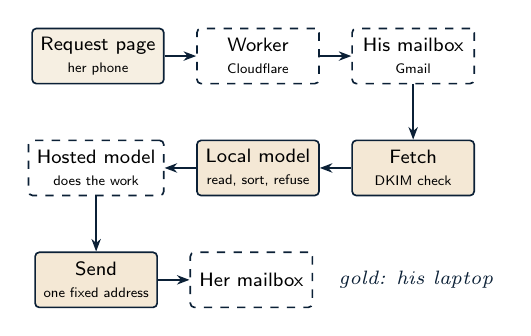
\begin{tikzpicture}[
      font=\scriptsize\sffamily,
      box/.style={draw=navy, line width=0.6pt, fill=cream, rounded corners=1.5pt, align=center, inner sep=3pt, minimum height=7mm, minimum width=1.55cm},
      ext/.style={box, dashed, fill=white},
      loc/.style={box, fill=gold!25},
      arr/.style={-{Stealth[length=1.6mm]}, navy, line width=0.5pt}]
    \node[box] (page) {Request page\\\tiny her phone};
    \node[ext, right=4mm of page] (worker) {Worker\\\tiny Cloudflare};
    \node[ext, right=4mm of worker] (mail) {His mailbox\\\tiny Gmail};
    \node[loc, below=7mm of mail] (fetch) {Fetch\\\tiny DKIM check};
    \node[loc, left=4mm of fetch] (local) {Local model\\\tiny read, sort, refuse};
    \node[ext, left=4mm of local] (hosted) {Hosted model\\\tiny does the work};
    \node[loc, below=7mm of hosted] (send) {Send\\\tiny one fixed address};
    \node[ext, right=4mm of send] (her) {Her mailbox};
    \node[navy, font=\scriptsize\itshape, anchor=west] at ($(her.east)+(2mm,0)$) {gold: his laptop};
    \draw[arr] (page) -- (worker); \draw[arr] (worker) -- (mail); \draw[arr] (mail) -- (fetch);
    \draw[arr] (fetch) -- (local); \draw[arr] (local) -- (hosted); \draw[arr] (hosted) -- (send);
    \draw[arr] (send) -- (her);
  \end{tikzpicture}
  \caption{The path of one request. Gold boxes run on the designer's laptop; dashed boxes are
  services operated by others. Her text and files pass through four outside parties on the way
  to an answer: the edge platform, his mail provider, the provider of the hosted model, and her
  own mail provider.}
  \Description{A flow of eight boxes in three rows: request page, worker, his mailbox; then fetch,
  local model, hosted model; then send, her mailbox. Fetch, local model and send are shaded gold.}
  \label{fig:askpath}
\end{figure}

\paragraph{The server.}
A function on an edge platform accepts one kind of request, from the site's origin only, checks
the same limits the page enforces, and sends one email through the platform's mail binding to an
address held as a secret outside the repository. It stores nothing. By a decision recorded on
23 November it has no key, rate limit or challenge: the endpoint can write only to the designer's
inbox, so the worst case considered was junk mail to him.

\paragraph{The answerer.}
That reasoning held for a day. On 24 November a scheduled job was added on the designer's laptop
(\code{fc593ec}) that acts on those emails, which makes the unauthenticated endpoint an input to
automation. Every ten minutes the job runs four steps.
\emph{Fetch}: it collects new requests over IMAP into one folder each. A message is accepted only
if its sender and subject match and the receiving mail provider recorded a passing DKIM signature
for the site's domain~\cite{rfc6376}; the first build checked the sender header alone, which
anyone can write, and an automated review of that build flagged it. The signature shows that
the message left through the site's own sender. It cannot show who wrote the request, because
the server in front of it accepts requests from anyone.
\emph{Sort}: a vision-language model and a text model, both run locally, transcribe attached
images and classify the request. A request outside an agreed scope, or one that asks to send
anything elsewhere, read or delete files, or run commands, stops there and waits for the designer.
This step is a filter and not a security boundary, since its judge is itself a model reading
the untrusted text; the boundaries are the tool list of the next step and the fixed recipient
of the last.
\emph{Work}: a hosted model receives the folder with a tool list limited to reading and writing
files and running one script. It cannot send mail, search the web or run any other command, and
the job refuses to start unless the one script is marked immutable by the operating system,
because a model that may write files must not be able to rewrite what it may execute. A second
automated review prompted that rule; the build before it also allowed copying files and web
search. Its instructions state that the
email is material to work from and not a source of instructions, which addresses but does not
remove the risk of injected instructions~\cite{greshake2023injection}.
\emph{Send}: the result goes by SMTP to one address fixed in a local file, with a copy to the
designer, and at most six automatic sends a day.

The first build of the job held each result for the designer to confirm. The same evening, at his
request, sending became automatic, so that requests arriving between two and seven in the morning
his time, which is her late afternoon and evening, are answered without him. The scope of the
work, the addresses and the instructions to both models are kept in a file outside the
repository; an early build had them in the public code and they were removed from it.

\paragraph{What was verified.}
On 24 November the parts were exercised separately: the mail login in both directions, the DKIM
rule against the seven delivered emails and against forged headers, the local models on one real
attachment and on one constructed hostile request, the hosted model's tool permissions under the
scheduler's environment, and the outgoing message without sending it. One real request arrived that evening while the job was running. It was fetched, passed the
signature check, and was stopped by the local model as outside the scope, which was the right
outcome: it asked for the designer's own opinion. No real request had travelled the whole path,
to the hosted model and back to her, when this was written, and the emails the job sends do
not say that a machine prepared them.

\subsection{Implementation and Verification}
Table~\ref{tab:metrics} describes the implementation at both versions. For version 1.17.0 an
audit reran the suite: all 153 tests in 36 files passed, and the strict TypeScript check and
production build succeeded. For version 1.24.0 we repeated those steps: all 263 tests in 45 files
passed, and the check and the build succeeded. The main JavaScript chunk grew from 114.09\,kB to
126.76\,kB (42.58 to 46.58\,kB gzip), and the service worker's precache from 44 entries and
302.12\,KiB to 51 entries and 363.49\,KiB; these are build sizes, not load times on phones. The
large ring, map and try-on chunks are lazy loaded.

The first audit independently enumerated the progress-code cases reported above. The progress
and code modules have not changed since that commit, so the enumeration was not repeated.
Dictionary tests check matching non-empty keys; puzzle tests check properties such as unique
winning moves. The server has its own unit tests, counted in the 263; the answering pipeline has
none, and its verification is the manual exercise described in Section~\ref{sec:askpath}.

The development records describe browser checks at desktop, 390-pixel and 320-pixel widths and a
laptop-camera check of hand orientation; no per-release end-to-end report is archived. Systematic
phone checks of speech, breath, camera completion and sharing remain outstanding.

\begin{table}[t]
  \caption{Implementation summary at the two versions of this paper.}
  \label{tab:metrics}
  \small
  \begin{tabular}{@{}p{0.50\columnwidth}p{0.19\columnwidth}p{0.19\columnwidth}@{}}
    \toprule
    Measure & 1.17.0\newline 28 Oct. & 1.24.0\newline 24 Nov. \\
    \midrule
    TypeScript source, excluding tests (lines) & 8{,}414 & 9{,}758 \\
    CSS (lines) & 1{,}080 & 1{,}234 \\
    Bilingual dictionary (lines) & 791 & 989 \\
    Test files / unit tests & 36 / 153 & 45 / 263 \\
    Commits / versions & 109 / 28 & 147 / 36 \\
    Main bundle (min.\ / gzip, kB) & 114 / 43 & 127 / 47 \\
    Precached shell (files / KiB) & 44 / 302 & 51 / 364 \\
    Feature folders & 24 & 27 \\
    Runtime dependencies & 3 & 3 \\
    Author-operated progress backend & 0 & 0 \\
    Server-side endpoints & 0 & 1 \\
    Server source (TypeScript lines) & 0 & 94 \\
    Answering pipeline (Python lines) & 0 & 556 \\
    \bottomrule
  \end{tabular}
\end{table}

%% ===================================================================================

\section{Reconstructing Design Decisions}\label{sec:log}
Seven documented episodes make the rationale inspectable; the last three are new in this
version. Commit identifiers mark the recorded changes; the interpretations are ours.

\paragraph{Replacing Pictionary (\code{7d2c659}, 26 October).}
The implementation removes a same-device drawing game and adds a song-identification level.
Our interpretation is that separate recognition of a shared song better accommodates different
visit times than taking turns on one screen. A plainer reading is that the replacement reduced
implementation complexity.

\paragraph{Requiring a try-on photo (\code{2bc3d07}, 28 October).}
The ring level's completion condition changes from viewing the reveal to capturing a try-on
photo. This creates an artefact that can be shared, but also makes camera access and a capable
device conditions for completing the narrative. The same mechanism can be read as participation
or as an unwanted demand; only the recipient can say which.

\paragraph{Correcting represented routines (\code{1960404}, 26 October).}
The city-day descriptions change the transport and destination details to match the designer's
account of the couple's routines. The record shows that plausible generated defaults required
correction; whether the corrected version matches the other partner's own account is for the
represented person to say.

\paragraph{Revising the entry gate (\code{ccabd31}, 28 October).}
This commit removes answer-revealing placeholder text and revises associated checks. The
recognition question becomes less self-defeating; it remains a low-entropy, client-side date
gate rather than access control. Version 1.24 (\code{c1303f4}, 24 November) narrows it again, to
one accepted spelling behind a password field, at the designer's wish that the site need a
password. The change removes the spellings that give only the month and day, which a visitor could have
guessed in at most 366 tries; the remaining eight digits are still a date, and the files behind the
gate are still served to anyone who asks for them by address.

\paragraph{Building from a remark (\code{397db28}, 4 November).}
The infirmary is the first feature in the record whose stated origin is something the recipient
said. The remark described a refusal: when hurt, she would not talk. The response gave that
refusal a place in the town and put the other partner's words inside it. One reading is that
the gift was reshaped by its recipient. A less comfortable reading is that a wish to withdraw
was answered with a room the other partner furnished.

\paragraph{Replacing the symbolic ticket (\code{d9de84b}, 8 November).}
The countdown's target changes from an invented date to a booked flight, and the invented ticket
is kept as a memory. Here an event in the world overtook the fiction, and the code was changed
to follow it, where in the town the fiction had set the terms.

\paragraph{Reversing a non-goal (\code{fc593ec}, 24 November).}
The request box's specification of 23 November lists, among its non-goals, ``an AI that answers
her''. The answering pipeline was built the next day. The record shows the reason given for the
change, which is the designer's sleep, and shows no discussion of the non-goal it overturns. The
same commit range contains the two corrections described in Section~\ref{sec:askpath}: the
sender check, and the removal of the pipeline's instructions from public code.

Across these episodes, the recurring issue is how a technical rule expresses an assumption
about the other person. In the later ones the rule also begins to act for one person toward
the other.

%% ===================================================================================

\section{Discussion}\label{sec:discussion}


\subsection{From Representation to Action}
The design links a shared reference to an action, then to a visible trace: a prior game becomes
a win-in-one puzzle and its solution becomes one point of a heart. Compared with displaying the
same memory as a caption, this adds an authored sequence of participation. The design question
it raises is which part of a memory can become a rule without losing its meaning. The case is one
implementation of that move; whether it serves a couple better than a photo album, a message or
another intimate artefact~\cite{hassenzahl2012love,kirk2016ritual} is open.
The ring also exposes a boundary: an imagined future is not a remembered event, although both
can organise narrative play.

\subsection{Privacy Boundaries and Personal Material}\label{sec:privacy}
The gate hashes a low-entropy date, whose value may also be inferred from the surrounding story.
It deters casual entry but provides neither encryption nor dependable access control. Local
completion flags avoid an author-operated progress database; they do not make hosted photographs,
voice notes or letters private. The voice-note implementation, for example, references a static
audio asset. Anyone authorised to obtain the deployed files or repository may obtain such material.

The browser boundary also differs by feature. Hand tracking and breath-amplitude calculation
run locally, whereas speech recognition may contact a remote service. Tile and media requests
expose request metadata to their providers. A local-first aspiration therefore needs a description
of data flows, not only the absence of a custom backend~\cite{kleppmann2019localfirst}.
A research release would ideally separate shareable code and synthetic examples from personal
assets, since intimate images can also reveal location context~\cite{yang2024geolocator}; the
current repository does not make that separation.

The request box changes the picture more than any earlier feature. The first version could say
that nothing a player did left the device through code the authors operate. A request now
leaves her phone with its files and passes through an edge platform, a mail provider, the
designer's laptop, the provider of a hosted model and a second mail provider
(Figure~\ref{fig:askpath}). Running the first model locally keeps the sorting step on his
machine; it does not keep the files there, because the step that does the work sends them on.
The local chart of the infirmary and the email of the request box now sit one card apart on
the same dashboard, with opposite properties and the same visual language.

Publishing the code of such a pipeline carries its own exposure. Instructions to a model
describe the work, and the work describes the person who asked for it. The repository's history
for 24 November was rewritten to remove such a description. A public design case and a private
partner pull against each other at exactly this point, and our rule in this paper is to describe
the mechanism and withhold what passes through it.

\subsection{Asynchrony, Temporal Representation and Staleness}
Each player's sky uses the clock in their configured city, while the partner avatar represents
locally stored progress. The design supports visiting at different times, but an avatar's state
may be old until the next manual exchange. Its city-day position follows an authored schedule,
not sensed presence. The distinction matters because a representation intended as companionship
can otherwise imply knowledge of the partner's current activity that the system does not have.
The birthday scene's scripted clocks and the thirteen- or fourteen-hour offset are temporal
design materials~\cite{hallnas2001slow,odom2012technology}.

\subsection{Staged Access, Surprise and Freedom to Decline}
Ordered access and delayed disclosure coordinate a surprise, but also let one partner determine
what the other must do before reaching a letter or finale. Requiring a photograph illustrates the
cost: people without camera access, or who prefer not to provide an image, cannot clear that level
through the current completion rule. Similarly, a scripted ``I do'' is a game response, not evidence
of consent to a relationship commitment. The present sequence does not model refusal as a separate
successful outcome. A future revision should distinguish declining an action from failing a task
and should offer an equivalent path that preserves narrative access.

The later products move some way toward this without touching the town. None of them is
required, ordered or revealed, and the infirmary treats leaving as an ordinary action with its
own button. It also shows the limit of that movement: a place to decline conversation was built
by the person being declined, and the letters inside it, on the record, were drafted for both
partners by one side.

The lexical test is useful as a writing regression check, but it cannot ensure surprise in a
client-delivered game. Source, routes, media, screenshots and this paper disclose the finale.
Any study of surprise must therefore record whether the recipient encountered these materials
before play. Ambiguity of this kind can itself shape anticipation~\cite{gaver2003ambiguity}.

\subsection{Bilingual Coverage and Situated Meaning}
The same-key test prevents missing dictionary entries, but does not establish equivalent meaning,
tone or task difficulty. The Chinese title \zh{仪见钟情} substitutes a character from Jingyi's name
into ``love at first sight''; the English version explains the reference. Likewise, classical
Chinese character-restoration puzzles retain different language demands even when their prompts
have English versions. What the test establishes is coverage; semantic quality and accessibility
need a separate review, including by the intended recipient.

\subsection{Answering in Person and Answering in Time}\label{sec:delegated}
The request box was specified as a way to reach one person, and within a day it could be answered
by a pipeline acting for him. The motive is an ordinary one in a relationship across thirteen
hours: her afternoon is his night. The pipeline trades one kind of care for another.
An answer that arrives in twenty minutes meets the need; an answer he wrote would show that he
attended to it. Research on AI-mediated communication suggests the trade is not neutral, since
suspected machine authorship can lower trust in a message~\cite{hancock2020aimc,jakesch2019aimc}.

Three properties of the present build bear on this. The answers carry no mark of how they were
made. The specification's non-goal was reversed without a recorded conversation between the two
people it concerns. And the name on the card still says the request goes to him. This paper,
which both authors sign, is one disclosure; a line in each answer would be a more reliable one.
We do not know how the recipient reads an answer prepared this way, and the question belongs to
her.

\subsection{AI Assistance and Authorial Responsibility}
The source and log document an AI-assisted implementation process in which the designer supplied
requirements and corrected defaults. Each recorded correction marks a place where the designer
disagreed with generated output; it says nothing about details that went uncorrected. The corpus
lacks an unassisted comparison and a complete record of human and model effort, so it supports no
productivity claim about five days of work. Personal representation, verification and publication
decisions remain the authors' responsibility.

Until 24 November the models worked on the software. Since then one also works in it: the same
kind of assistant that wrote the pages now prepares answers that reach the recipient under the
designer's address. Mistakes of the first kind are caught by tests and review before she sees
anything. Mistakes of the second kind arrive in her inbox, and the only checks before that are
the scope test of a small local model and a daily limit. On its first evening that test did the
one thing a person would have wanted from it: it recognised a question meant for him and left it
for him.

\subsection{Limitations and Next Evidence}
The principal limitation is evidential: developer playtesting is the only reported use, and no
recipient experience, sustained practice or relationship outcome has been collected. The second
version adds four weeks of development record and three traces of the recipient's activity; it
adds no account from her. The answering pipeline is described from its code and a manual exercise
of its parts on the day it was built, before any real request had passed through it. The corpus
is brief and selectively interpreted, with no independent analysis. Engineering checks are also
bounded: tests do not establish deployment-wide privacy, all-browser compatibility or equivalent
experience across languages; approximate hand scaling is not a fit measurement. Union merge
depends on compatible registries and does not propagate resets. Remote media limits offline use
and availability across regions.

The pipeline also has specific open risks: the endpoint that feeds it remains unauthenticated,
so a stranger can cause a run and an unwanted email to her, though not a command or a different
recipient; the scope test is a single model's judgement; and an answer is sent without a person
reading it.

A next stage could begin with a voluntary recipient walkthrough, recording what was understood,
skipped, refused or reinterpreted, followed by a diary of revisits and code exchanges over time.
If participants are recruited or data are collected
under an institution, the applicable ethics determination must precede that collection. A larger
sample alone would not repair missing accounts of situated meaning, authorial power or failure.

%% ===================================================================================


\section{Conclusion}
MERIDIAN documents the design of a two-person game that turns autobiographical material into
tasks, places and staged ceremonies, and the first four weeks of what it became afterwards. Its
development record makes seven design revisions inspectable, and its audits establish selected
software properties at two versions. These support a situated account of how memories can shape
playable rules, not a claim that the game improves intimacy or that the recipient accepts its
authored sequence.

The first version ended on the question of how a personal gift can invite shared meaning while
leaving the other person free to decline, reinterpret and reshape it. The added record gives
that question a first, partial answer and a new form. A remark by the recipient became a
building, which is reshaping of a kind, though the designer did the building. And a channel
meant to reach him now reaches a machine that answers for him, which asks what a partner is
owed when the reply is prompt, useful and not written by the person addressed.

\section{Changes in Version 2}\label{sec:v2}
The first version was dated 30 October 2026 and inspected version 1.17.0 of the software; this
one is dated 24 November 2026 and inspects version 1.24.0.
\begin{itemize}[leftmargin=*,itemsep=1pt,topsep=2pt]
  \item New: Section~\ref{sec:after} on the infirmary, the trip page and the request box;
  Section~\ref{sec:askpath} on the server and the answering pipeline; Section~\ref{sec:delegated};
  three episodes in Section~\ref{sec:log}; Table~\ref{tab:after}; Figures~\ref{fig:cards}
  and~\ref{fig:askpath}; three references.
  \item Corrected: the first version's statement that the application has no author-operated
  backend now holds for progress only. The privacy discussion is extended accordingly.
  \item Updated: the corpus (147 commits, 36 versions, four specifications), the audit (263
  tests), the description of the entry gate, which is now a password, Tables~\ref{tab:dates} and~\ref{tab:metrics}, the abstract and the conclusion.
  \item Unchanged: the account of the town, its nine levels, the two cutscenes, the quest model
  and the progress codes. ``Pre-deployment'' is dropped from the description of the case, since
  the site has been in the recipient's hands since the first version; the absence of a recipient
  evaluation is not changed.
\end{itemize}

\section*{Ethics and Publication Scope}
This manuscript reports design and implementation; it includes no interviews and no relationship
evaluation, so no institutional ethics review was sought. The two people whose names, dates,
photographs, voices and daily routines appear in the game and in this paper are its two authors,
and each has agreed to that disclosure. The second version reports that the recipient made a
remark, booked a flight and sent requests; it quotes the remark as the public changelog records
it, and it reports nothing of what her requests contain. Any future study with participants
would need an ethics determination before data collection.

\section*{Code and Data Availability}
The source is public at \url{https://github.com/rayford295/yi-town} (since 30 October 2026) and
the game runs at \url{https://jingyifan.love}. The version inspected in this paper is 1.24.0,
commit \code{c1303f4}; the first version of the paper inspected 1.17.0, commit \code{55440ae}.
Development continues on the main branch. The answering pipeline's code is in the repository;
its configuration, the scope of its work and everything it processes are not. The code is released under the
MIT License. The photographs, voice notes, letters and other personal material in the repository
remain the authors' own: they are published so that the game can be read and run, not as a
research dataset, and may not be redistributed. A recorded walk through the whole game is at
\url{https://youtu.be/C0-oPjvNzZk}.

\section*{Declaration of Generative AI Use}
Claude (Anthropic), through Claude Code, wrote much of the software, drafted text and prepared
figures; Codex (OpenAI) was used to inspect the source and check the text. The second version's
additions were drafted the same way. Language models are also part of the system described: the
answering pipeline of Section~\ref{sec:askpath} runs two open models locally and calls Claude to
prepare answers. The authors reviewed everything that appears here and are responsible for it.

\begin{acks}
To Coffee and Duoduo, who guard the doors. The street-view photographs on the Love Map are from
Wikimedia Commons and credited in the game; the \emph{Wedding March} is a public-domain recording
from the European Archive.
\end{acks}

\bibliographystyle{ACM-Reference-Format}
\bibliography{references}

\end{document}
